\documentclass{beamer}
\usetheme{CambridgeUS}
\usecolortheme{seahorse}
\usefonttheme{serif} 
\usepackage[utf8]{inputenc}
%\usepackage{default}
\usepackage{booktabs}
\usepackage{pifont}
\usepackage{lineno}
%\usepackage{beamerthemesplit}
%\usepackage{stmaryrd}
\usepackage{comment}
\usepackage{subfig}
\usepackage[percent]{overpic}
\usepackage{amsfonts}
\usepackage{amsmath}
\usepackage{amssymb}
\usepackage{movie15}
\usepackage{mathrsfs}
\usepackage{fixltx2e}
\usepackage{lipsum}
\setbeamertemplate{caption}{\raggedright\insertcaption\par}
\newcommand\blfootnote[1]{%
  \begingroup
  \renewcommand\thefootnote{}\footnote{#1}%
  \addtocounter{footnote}{-1}%
  \endgroup
}


\newcommand{\argmin}[1]{\underset{#1}{\operatorname{arg}\,\operatorname{min}}\;}
\newcommand{\cmark}{\ding{51}}%
\newcommand{\xmark}{\ding{55}}%
\newcommand{\bAT}{\boldsymbol{AT}}
\newcommand{\bLS}{\boldsymbol{LS}}
\newcommand{\bl}{\boldsymbol{l}}
\newcommand{\bx}{\boldsymbol{x}}
\newcommand{\bs}{\boldsymbol{s}}
\newcommand{\by}{\boldsymbol{y}}
\newcommand{\bZ}{\boldsymbol{Z}}
\newcommand{\bc}{\boldsymbol{c}}
\newcommand{\bz}{\boldsymbol{z}}
\newcommand{\bX}{\boldsymbol{X}}
\newcommand{\bE}{\boldsymbol{E}}
\newcommand{\bF}{\boldsymbol{F}}
\newcommand{\bL}{\boldsymbol{L}}
\newcommand{\bO}{\boldsymbol{O}}
\newcommand{\bP}{\boldsymbol{P}}
\newcommand{\bQ}{\boldsymbol{Q}}
\newcommand{\bD}{\boldsymbol{D}}
\newcommand{\bC}{\boldsymbol{C}}
\newcommand{\bT}{\boldsymbol{T}}
\newcommand{\bW}{\boldsymbol{W}}
\newcommand{\bbeta}{\boldsymbol{\beta}}
\newcommand{\sX}{\mathcal{X}}
\newcommand{\sA}{\mathcal{A}}
\newcommand{\sY}{\mathcal{Y}}
\newcommand{\bSigma}{\boldsymbol\Sigma}
\newcommand{\bDelta}{\boldsymbol\Delta}
\newcommand{\bU}{\boldsymbol{U}}
\newcommand{\bV}{\boldsymbol{V}}
\newcommand{\bI}{\boldsymbol{I}}
\def\bA{\boldsymbol{A}}
\def\bY{\boldsymbol{Y}}
\def\bB{\boldsymbol{B}}
\def\bl{\boldsymbol{l}}

\newtheorem{bigthm}{Theorem}
\renewcommand{\thebigthm}{\Alph{bigthm}}	% Number with A, B, C, etc.

\newtheorem{thm}{Theorem}
\newtheorem{cor}[thm]{Corollary}

\newcommand{\argmint}{\operatorname*{arg\; min}}

\newcommand{\diag}{\operatorname{diag}}
\usepackage{algorithm}
\usepackage[noend]{algpseudocode}
\captionsetup[figure]{labelformat=empty}
\begin{document}

\title[FPO Talk]{Image Restoration and 3D Reconstruction from Cryo-EM Images}
\institute[
]
{
Final Public Oral Exam, Princeton University\\
Advisers: Amit Singer and Joshua Shaevitz} 
\date{May 9, 2017} 
\author{Tejal Bhamre}

\begin{frame}
\titlepage 
\end{frame}

\begin{frame}{Outline}
\tableofcontents
\end{frame} 


\AtBeginSection[]{
  \begin{frame}
  \vfill
  \centering
  \begin{beamercolorbox}[sep=8pt,center,shadow=true,rounded=true]{title}
    \usebeamerfont{title}\insertsectionhead\par%
  \end{beamercolorbox}
  \vfill
  \end{frame}
}

 
\section{Introduction}

\begin{frame}<beamer>
\setbeamercovered{transparent}
\frametitle{Cryo-Electron Microscopy (Cryo-EM)}
\begin{columns}
\column{0.5\linewidth}
\centering
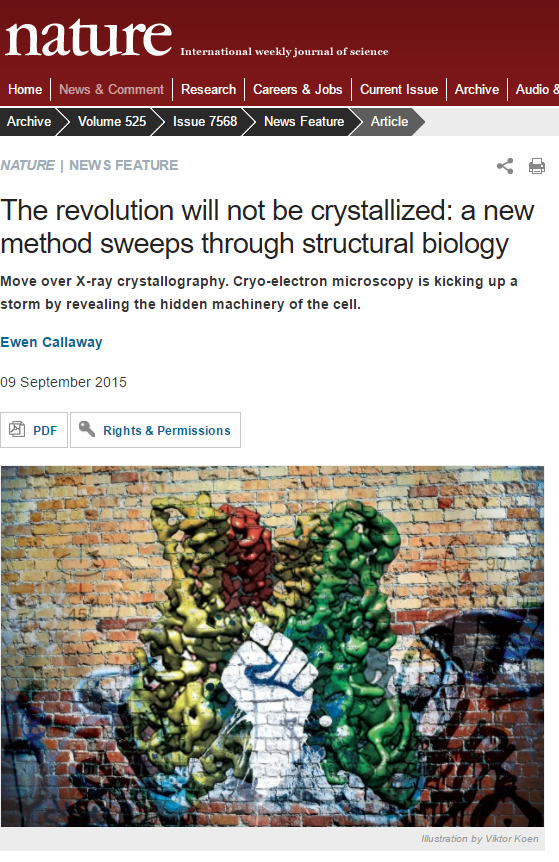
\includegraphics[scale=0.35]{figures/nature_news.png}
\column{0.5\linewidth} 
\begin{itemize}
\item Understanding function, mechanisms, drug discovery
\item X-ray crystallography has limitations
\item Structure of biological macromolecules \textit{in-vivo}, without crystallization
\item Reveal structural/ conformational variability
\end{itemize}
\end{columns}
\end{frame}


\begin{frame}<beamer>
\setbeamercovered{transparent}
\frametitle{Cryo-EM Revolution}
\begin{columns}
\column{1\linewidth} 
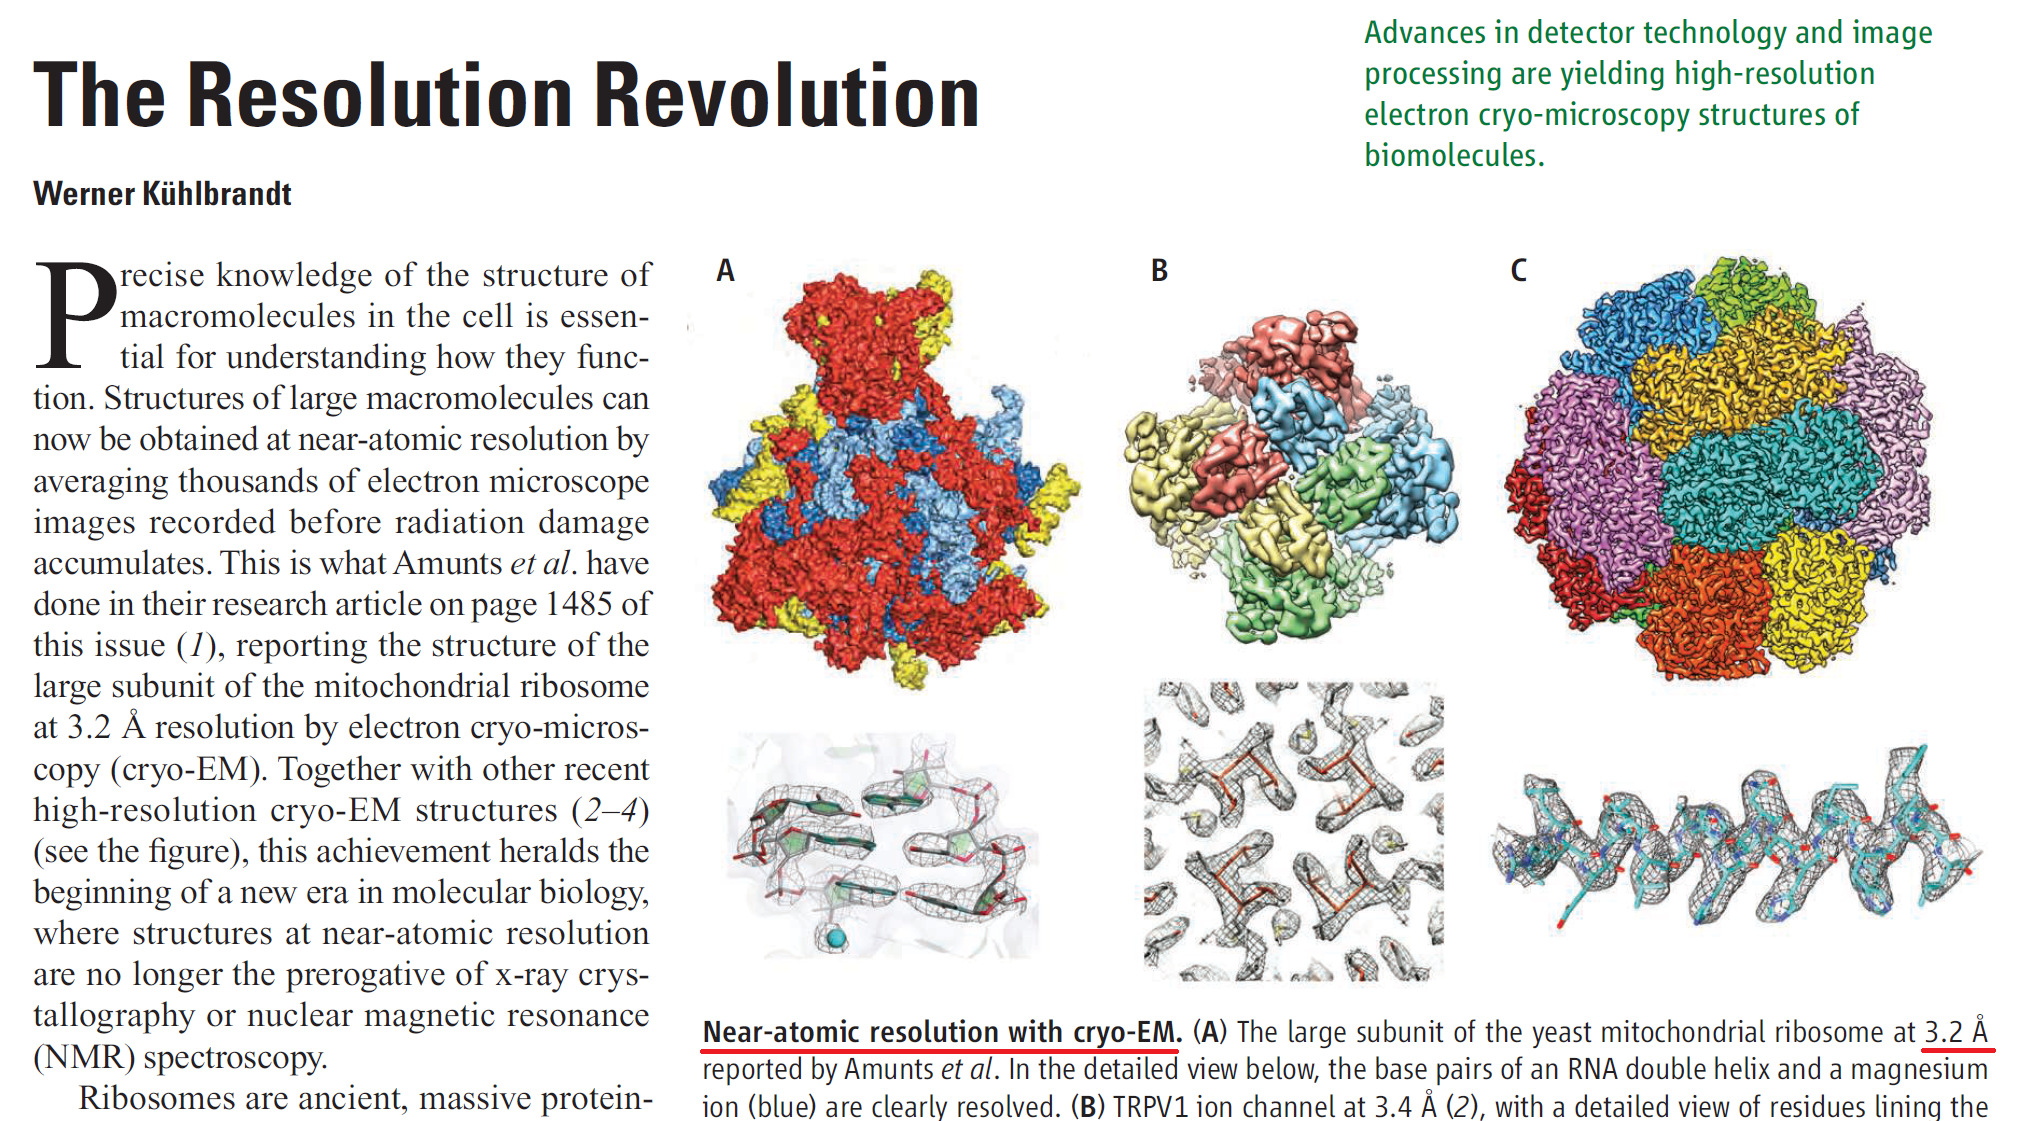
\includegraphics[scale=0.23]{figures/news2.png}
\end{columns}
\end{frame}


\begin{frame}<beamer>
\setbeamercovered{transparent}
\frametitle{Cryo-EM Database}
\begin{columns}
\column{1\linewidth}
\centering
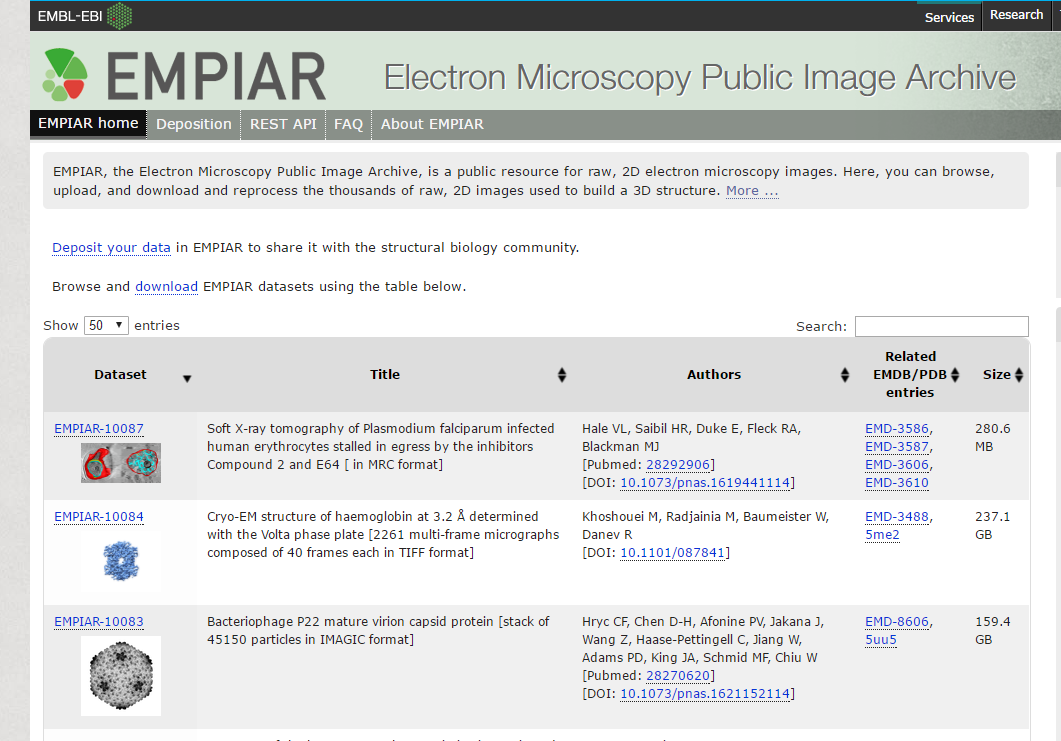
\includegraphics[scale=0.37]{figures/empiar_snap.png}
\end{columns}
\end{frame}

\begin{frame}<beamer>
\setbeamercovered{transparent}
\frametitle{Single Particle Reconstruction (SPR)}
\begin{columns}
\column{0.5\linewidth}
\centering
\begin{figure}
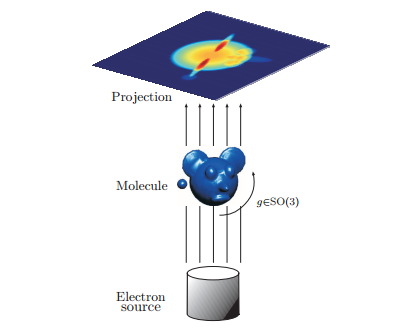
\includegraphics[scale=0.6]{figures/cryoem_imaging.png}
\caption{A. Singer et al. (2011)}
\end{figure}

\column{0.5\linewidth} 
\begin{itemize}
\item GOAL: 3D electron density map 
\item $\sim 10^5-10^6$ particles frozen in a thin, vitreous ice layer
\item Top view images with EM
\item Each particle assumes a random, unknown orientation
\end{itemize}
\end{columns}
%\blfootnote{A. Singer et. al. (2011)}
\end{frame}

\begin{frame}<beamer>
\setbeamercovered{transparent}
\frametitle{Single Particle Reconstruction (SPR)}
\begin{figure}[h]
\centering
{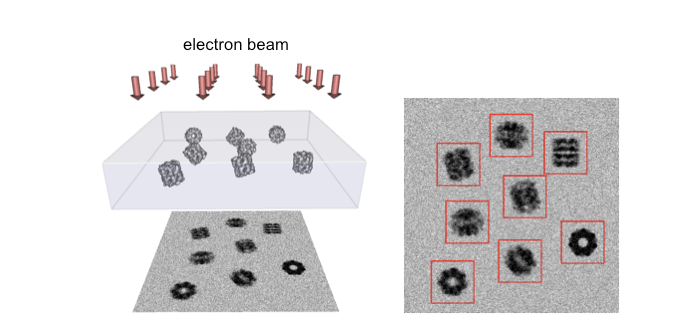
\includegraphics[scale=0.65]{figures/imaging_model.png}}
%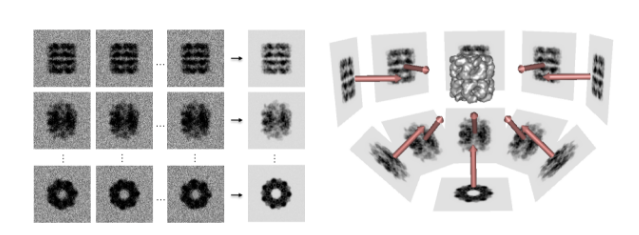
\includegraphics[scale=0.4]{figures/backproj.png}}
\label{fig:rawims}
\end{figure} 
\blfootnote{https://people.csail.mit.edu/gdp/cryoem.html}
\end{frame}


\begin{frame}<beamer>
\setbeamercovered{transparent}
\frametitle{Single Particle Reconstruction (SPR)}
\begin{figure}[h]
\centering
{%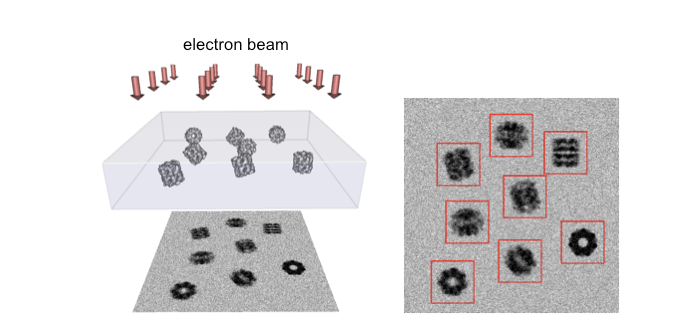
\includegraphics[scale=0.45]{figures/imaging_model.png}\\
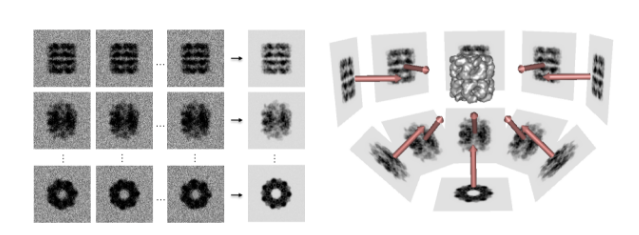
\includegraphics[scale=0.65]{figures/backproj.png}}
\label{fig:rawims}
\end{figure} 
\blfootnote{https://people.csail.mit.edu/gdp/cryoem.html}
\end{frame}


\begin{frame}<beamer>
\setbeamercovered{transparent}
\frametitle{Cryo-EM Length Scales}
\begin{columns}
\column{1\linewidth}
\centering
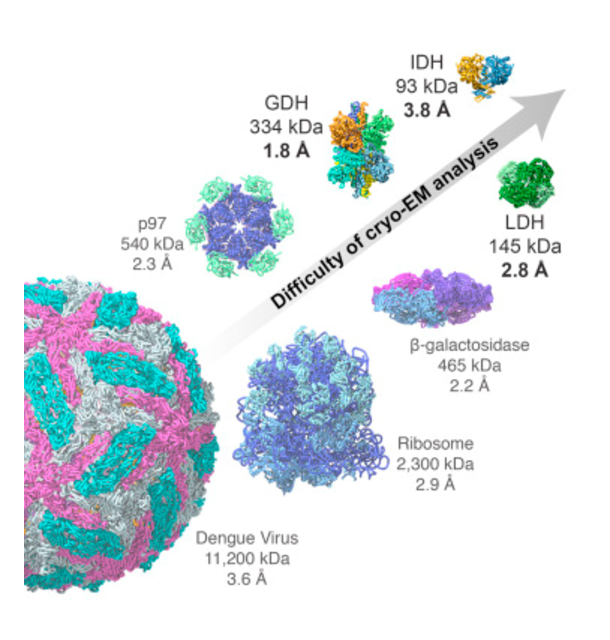
\includegraphics[scale=0.4]{figures/news_scales.png}
\end{columns}
\blfootnote{Merk et al. (2016)}
\end{frame}

\begin{frame}<beamer>
\setbeamercovered{transparent}
\frametitle{SPR Pipeline}
\begin{figure}[h]
\centering
{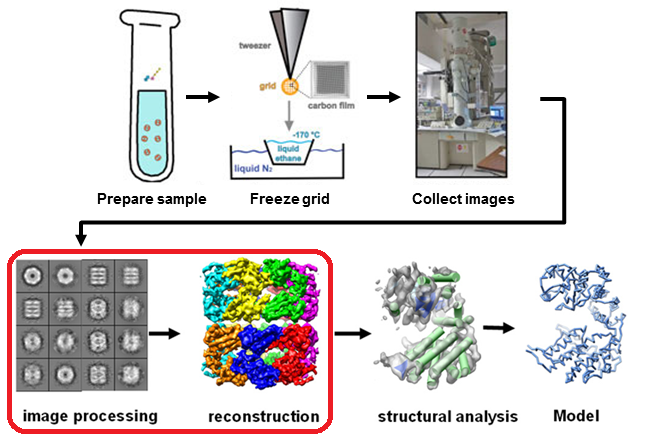
\includegraphics[scale=0.55]{figures/pipeline_pics.png}}
\label{fig:rawims}
\end{figure}
\blfootnote{Biomedical Image and Data Analysis Core}
\end{frame}

\begin{frame}<beamer>
\setbeamercovered{transparent}
\frametitle{Existing Computational Pipeline}
\begin{figure}[h]
\centering
{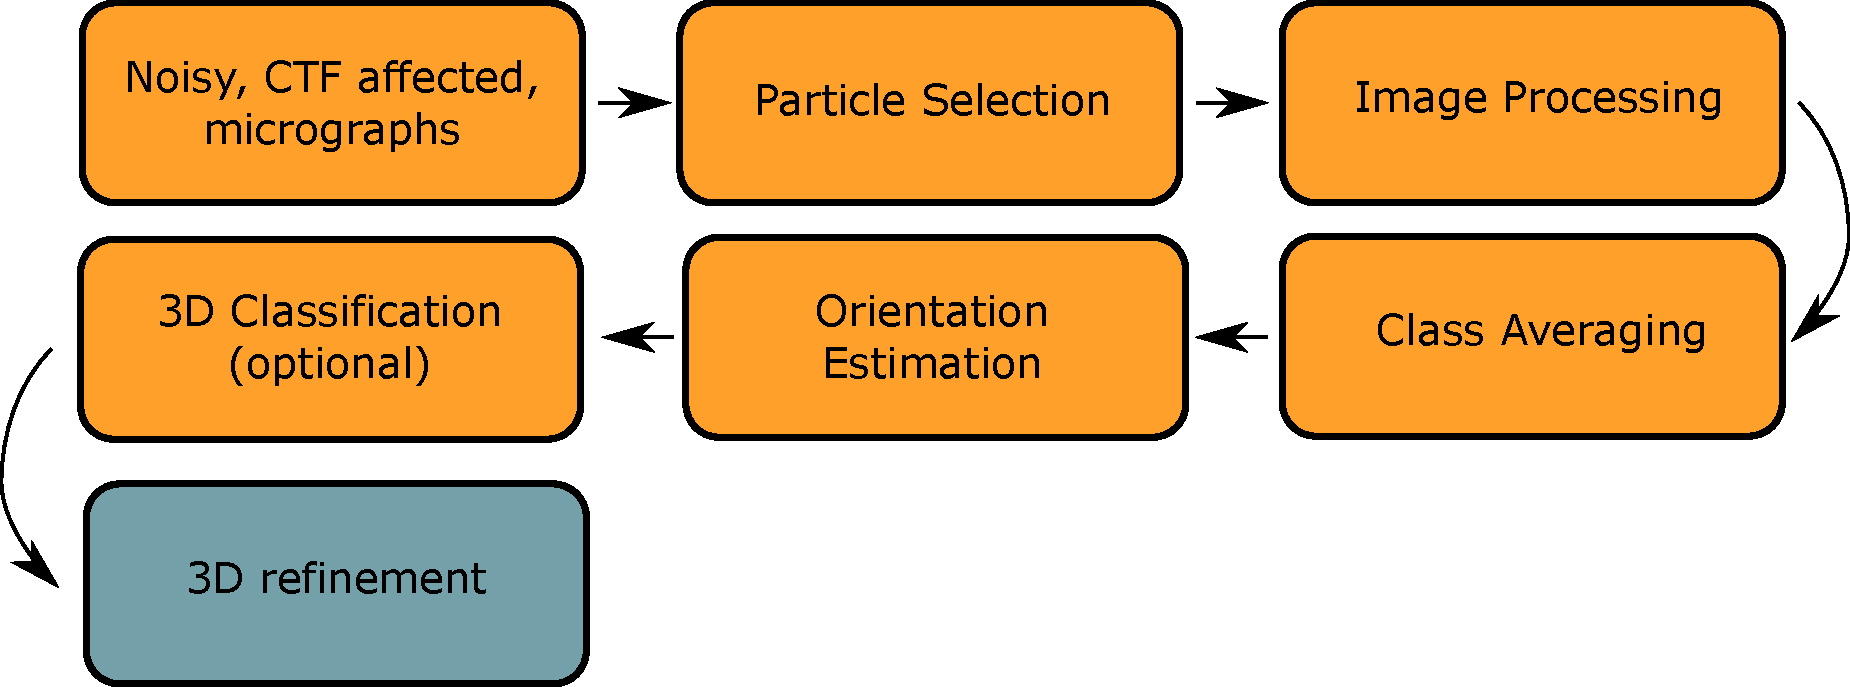
\includegraphics[scale=0.35]{figures/cryoem_pipeline_edited.pdf}}\\
\label{fig:rawims}
\end{figure}
\end{frame}

\section{Challenges and Contributions}

\begin{frame}<beamer>
\setbeamercovered{transparent}
\frametitle{Challenges}
\begin{figure}[h]
\centering
{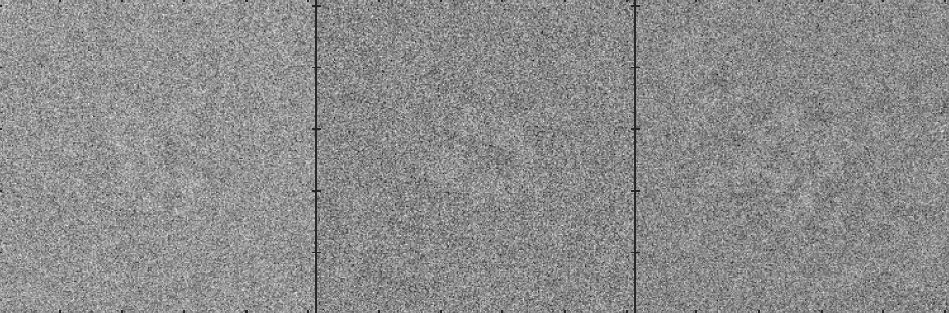
\includegraphics[scale=0.3]{figures/raw_expt_images.png}}\\
\label{fig:rawims}
\caption{Raw images from an experimental dataset of TRPV1  *\blfootnote{* EMPIAR-10059 }}
\begin{itemize}
 \item Radiation damage: very low signal to noise ratio (SNR)
 \item Information loss: contrast transfer function (CTF) of microscope
 \item Estimating unknown orientations of 2D images: challenging non-convex optimization
\end{itemize}
\end{figure}
\end{frame}

\begin{frame}<beamer>
\setbeamercovered{transparent}
\frametitle{Challenge: Covariance Estimation}
\begin{columns}
\column{1\linewidth} 
\begin{figure}
\centering
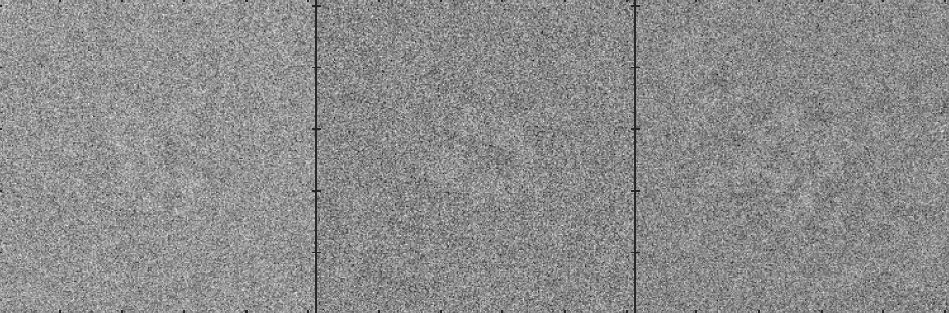
\includegraphics[width=.5 \columnwidth]{figures/raw_expt_images.png}
\end{figure}
\begin{itemize}
\item Existing CTF correction suboptimal
\item Need better denoising for preliminary inspection, outlier detection, without class averaging (expensive)
\item Covariance matrix estimate needed for denoising and our 3D homology approach
\end{itemize}
\end{columns}
\end{frame}


\begin{frame}<beamer>
\setbeamercovered{transparent}
\frametitle{Challenge: Initial Model for 3D Refinement}
\begin{columns}
\column{0.5\linewidth}
\begin{figure}
\centering
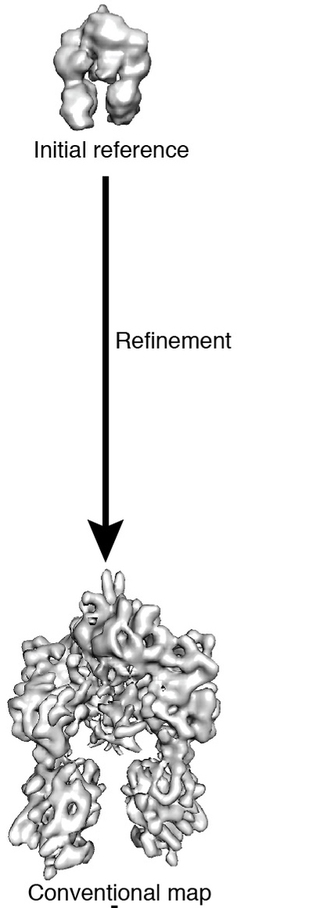
\includegraphics[width=.4 \columnwidth]{figures/refinement.png}\caption{S. Dutta et al.(2014)}
\end{figure}
\column{0.5\linewidth} 
\begin{itemize}
\item `Guess' low resolution initial model
 \item 3D refinement sensitive to initial model
 \item Data driven ab-initio model \blfootnote{ A. Singer et al. (2011)} using common-lines for orientation estimation
 \item Reliable estimation (common-lines etc.) difficult at low SNR without averaging
\end{itemize}
\end{columns}
\end{frame}


\begin{frame}<beamer>
\setbeamercovered{transparent}
\frametitle{Contributions}
\begin{enumerate}
\item \textbf{Covariance estimation from noisy, CTF affected images}
\begin{itemize}
\item Denoising and `optimal' CTF correction
\item Improve 2D classification
\item Outlier detection
\end{itemize}
\item \textbf{Homology modeling for 3D reconstruction}
\begin{itemize}
\item Reliable orientation estimation difficult at very low SNR
\item Need data-driven low resolution initial model
\item Use existing structures, \alert{skip 2D classification (averaging) and orientation estimation}
\end{itemize}
\end{enumerate}
Algorithms validated on both synthetic and real experimental datasets
\end{frame}

\begin{frame}<beamer>
\setbeamercovered{transparent}
\frametitle{Proposed Computational Pipeline}
\begin{figure}[h]
\centering
{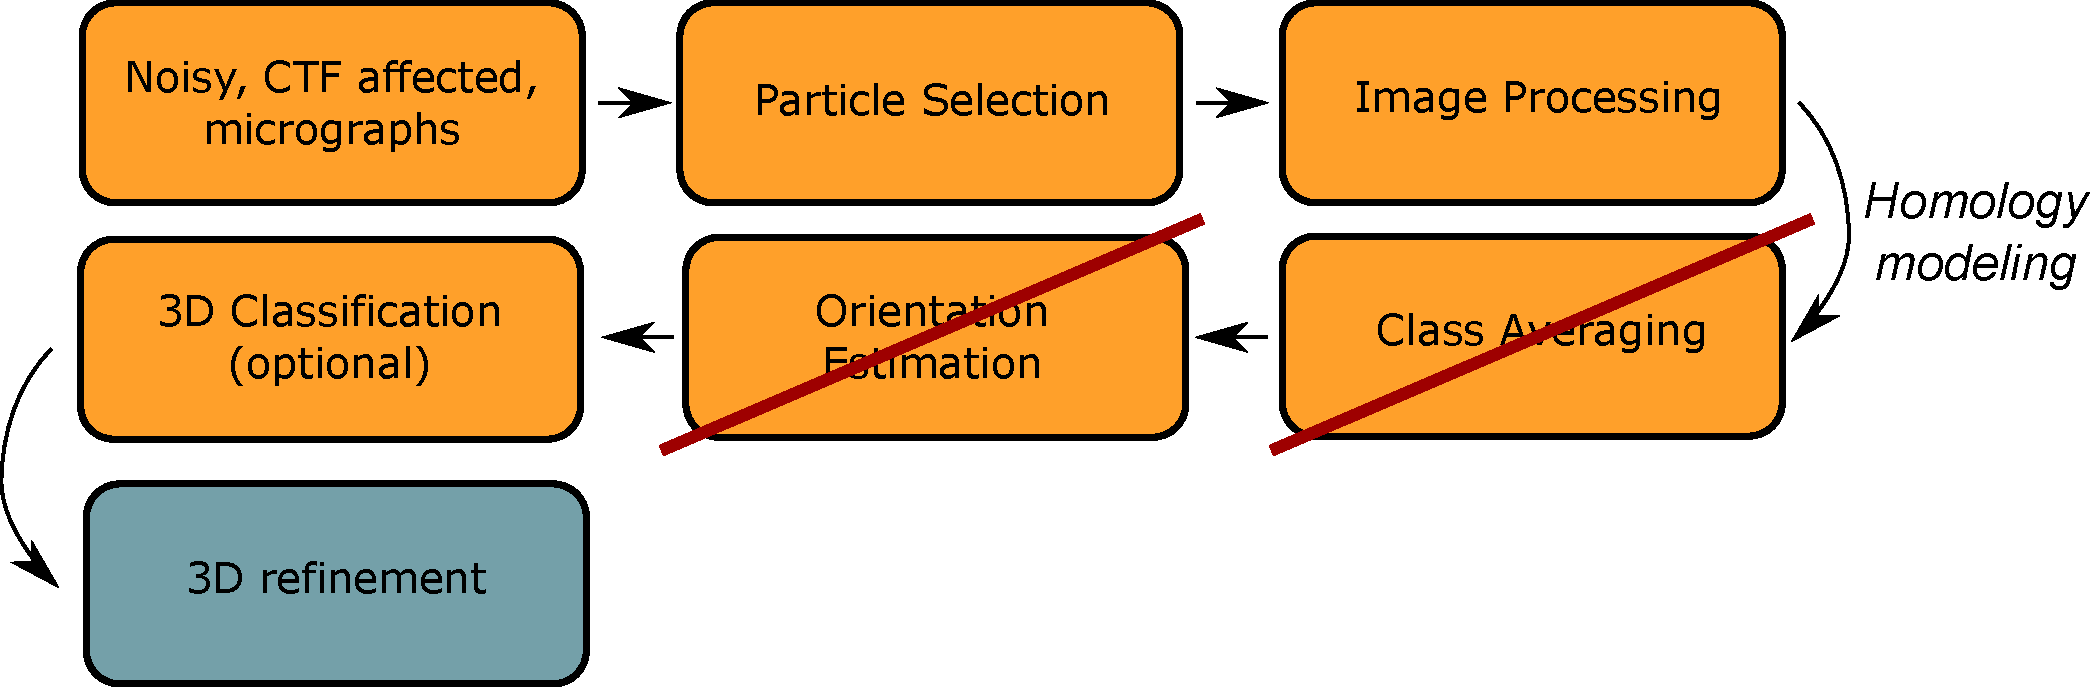
\includegraphics[scale=0.35]{figures/cryoem_pipeline_ours.pdf}}\\
\label{fig:rawims}
\end{figure}
\end{frame}


\begin{frame}<beamer>
\setbeamercovered{transparent}
\frametitle{Denoising: Real TRPV1 dataset}
\begin{columns}<+->
\column{0.2\linewidth}

\begin{figure}
\centering
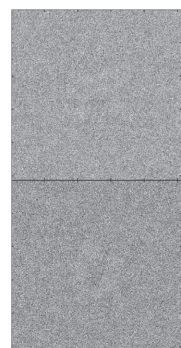
\includegraphics[width=.9 \columnwidth]{figures/deneg_raw.png}
\caption{Raw}
\end{figure}
\column{0.2\linewidth}

\begin{figure}
\centering
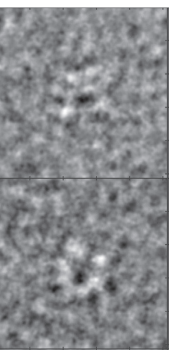
\includegraphics[width=.8 \columnwidth]{figures/deneg_twf.png}
\caption{Existing}
\end{figure}
\column{0.2\linewidth} 

\begin{figure}
\centering
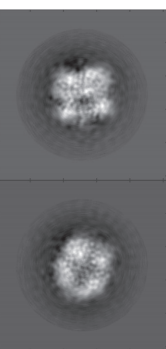
\includegraphics[width=.8 \columnwidth]{figures/deneg_cwf.png}
\caption{This work}
\end{figure}
\column{0.2\linewidth} 

\begin{figure}
\centering
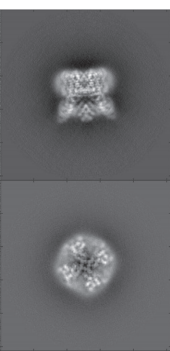
\includegraphics[width=.8 \columnwidth]{figures/deneg_clean.png}
\caption{Closest}
\end{figure}
\end{columns}
\blfootnote{T.B., T. Zhang, A. Singer (2016)}
\end{frame}


\begin{frame}<beamer>
\frametitle{Homology modeling: synthetic TRPV1 dataset}
\begin{figure}[!htbp]
\begin{tabular}{cc}
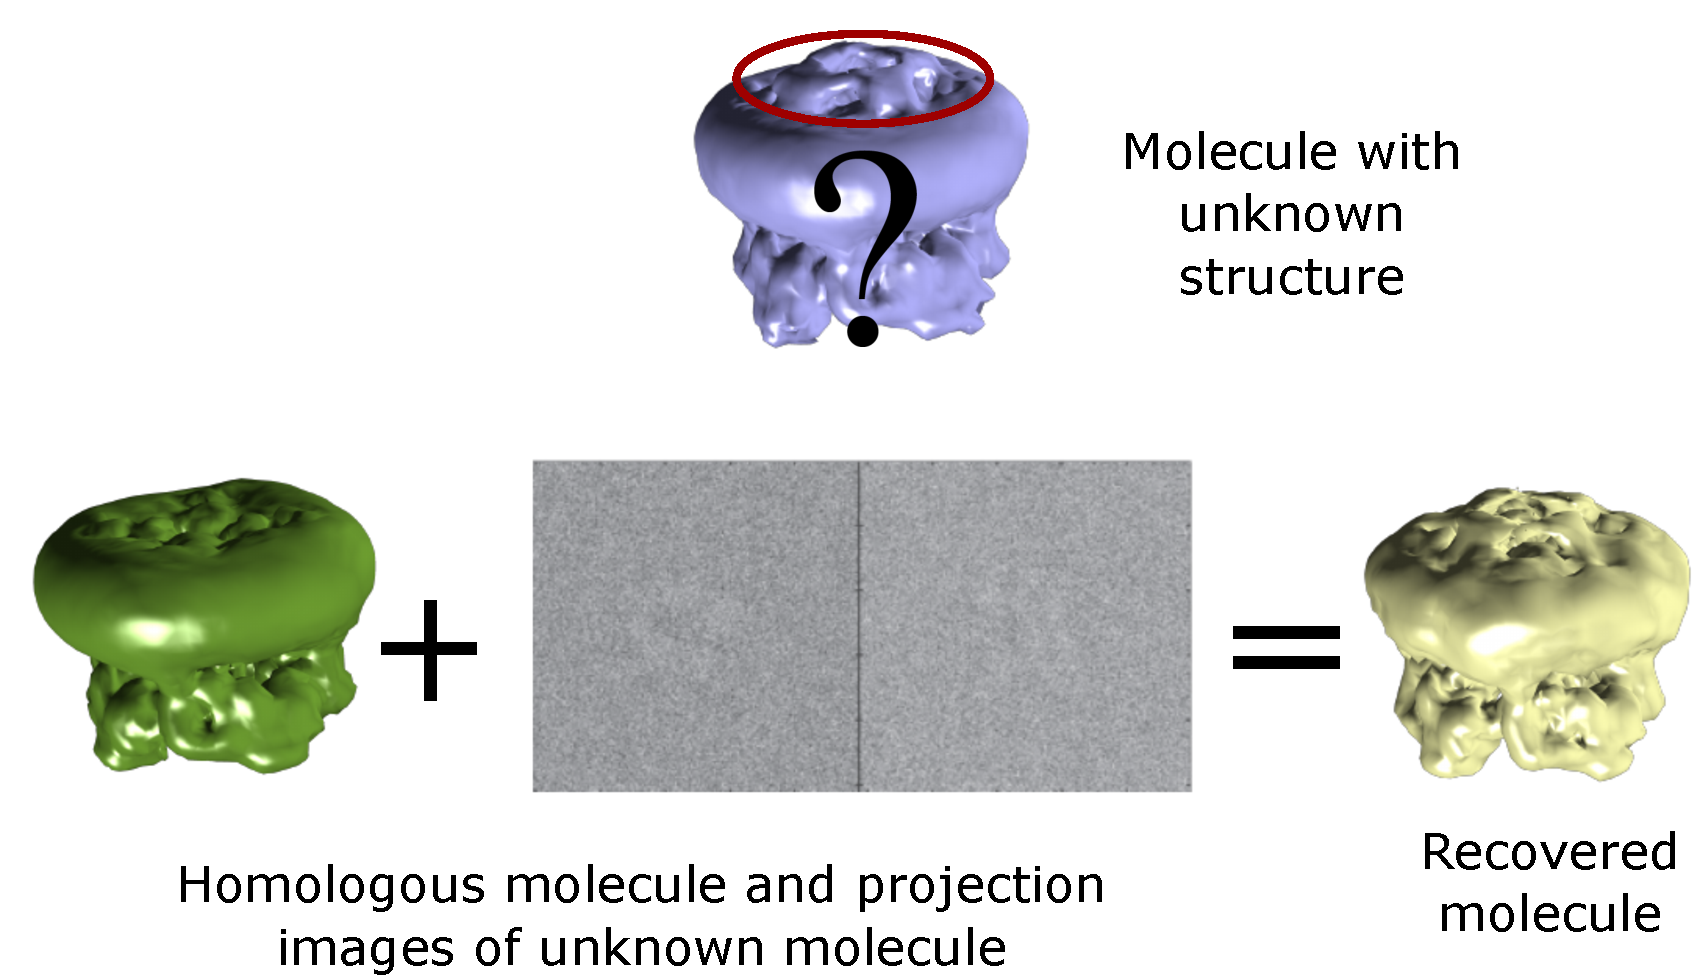
\includegraphics[width=0.95\linewidth]{figures/trpv1_flowchart.pdf}\label{fig:simtrpv_emdb}
\end{tabular}
\end{figure}\blfootnote{TB, T. Zhang, A. Singer (2017+), submitted}
\end{frame}

\begin{frame}<beamer>
\setbeamercovered{transparent}
\frametitle{Publications}
Work with Amit Singer, Jane Zhao, Teng Zhang\\
\begin{itemize}
\item \tiny{\textit{Orthogonal matrix retrieval in cryo-electron microscopy}, T.B., T. Zhang, and A. Singer, 12th IEEE International Symposium on Biomedical Imaging (2015)}

\item \tiny{\textit{Denoising and Covariance Estimation of Single Particle Cryo-EM Images}, T.B., T. Zhang, and A. Singer, Journal of Structural Biology (2016)}

\item \textit{Mahalanobis Distance for Class Averaging of Cryo-EM Image}, T.B., Z. Zhao, and A. Singer, 14th IEEE International Symposium on Biomedical Imaging (2017)

\item \textit{Anisotropic Twicing for Single Particle Reconstruction using Autocorrelation Analysis}, T.B., T. Zhang, and A. Singer, submitted (2017).

\end{itemize}
\end{frame}


\begin{frame}<beamer>
\setbeamercovered{transparent}
\frametitle{Code}
Open source software toolbox for cryo-EM: \url{spr.math.princeton.edu}
\begin{figure}\flushleft
\centering

\includegraphics[scale=0.45]{figures/aspire.png}
\end{figure}

\end{frame}

\section{Part 1: Covariance Estimation from Noisy, CTF Affected Images}
%
%\begin{frame}<beamer>
%\frametitle{Experimental data - TRPV1}
% 
%\begin{figure}[h]
%\centering
%{\begin{overpic}[width=0.5\textwidth]{figures/jsb_fig_tv.eps}%
%\put(10,77){\tiny Raw}
%\put(22,77){\tiny Closest projection}
%\put(59,77){\tiny TWF}
%\put(82,77){\tiny CWF}
%\end{overpic}
%\label{}}
%
%\label{fig:trpv1}
%\end{figure}
%% 
%\begin{itemize}
% \item K2 direct electron detector\\
% \item 35645 motion corrected, picked particle images of 256$\times$256 pixels
%\end{itemize}
%\end{frame}

\begin{frame}<beamer>
\setbeamercovered{transparent}
\frametitle{Motivation}
\begin{itemize}[]
 \item \textbf{Denoising}: visualize underlying particles without class averaging
 \item \textbf{Image restoration}: CTF correction and denoising in a single step
  \item \textbf{Automated outlier detection}
  \item Bonus: Improved class averaging
\end{itemize}
\end{frame}


\begin{frame}<beamer>
\setbeamercovered{transparent}
\frametitle{CTF Correction}
\vspace{-3mm}
\begin{figure}[]
%\centering
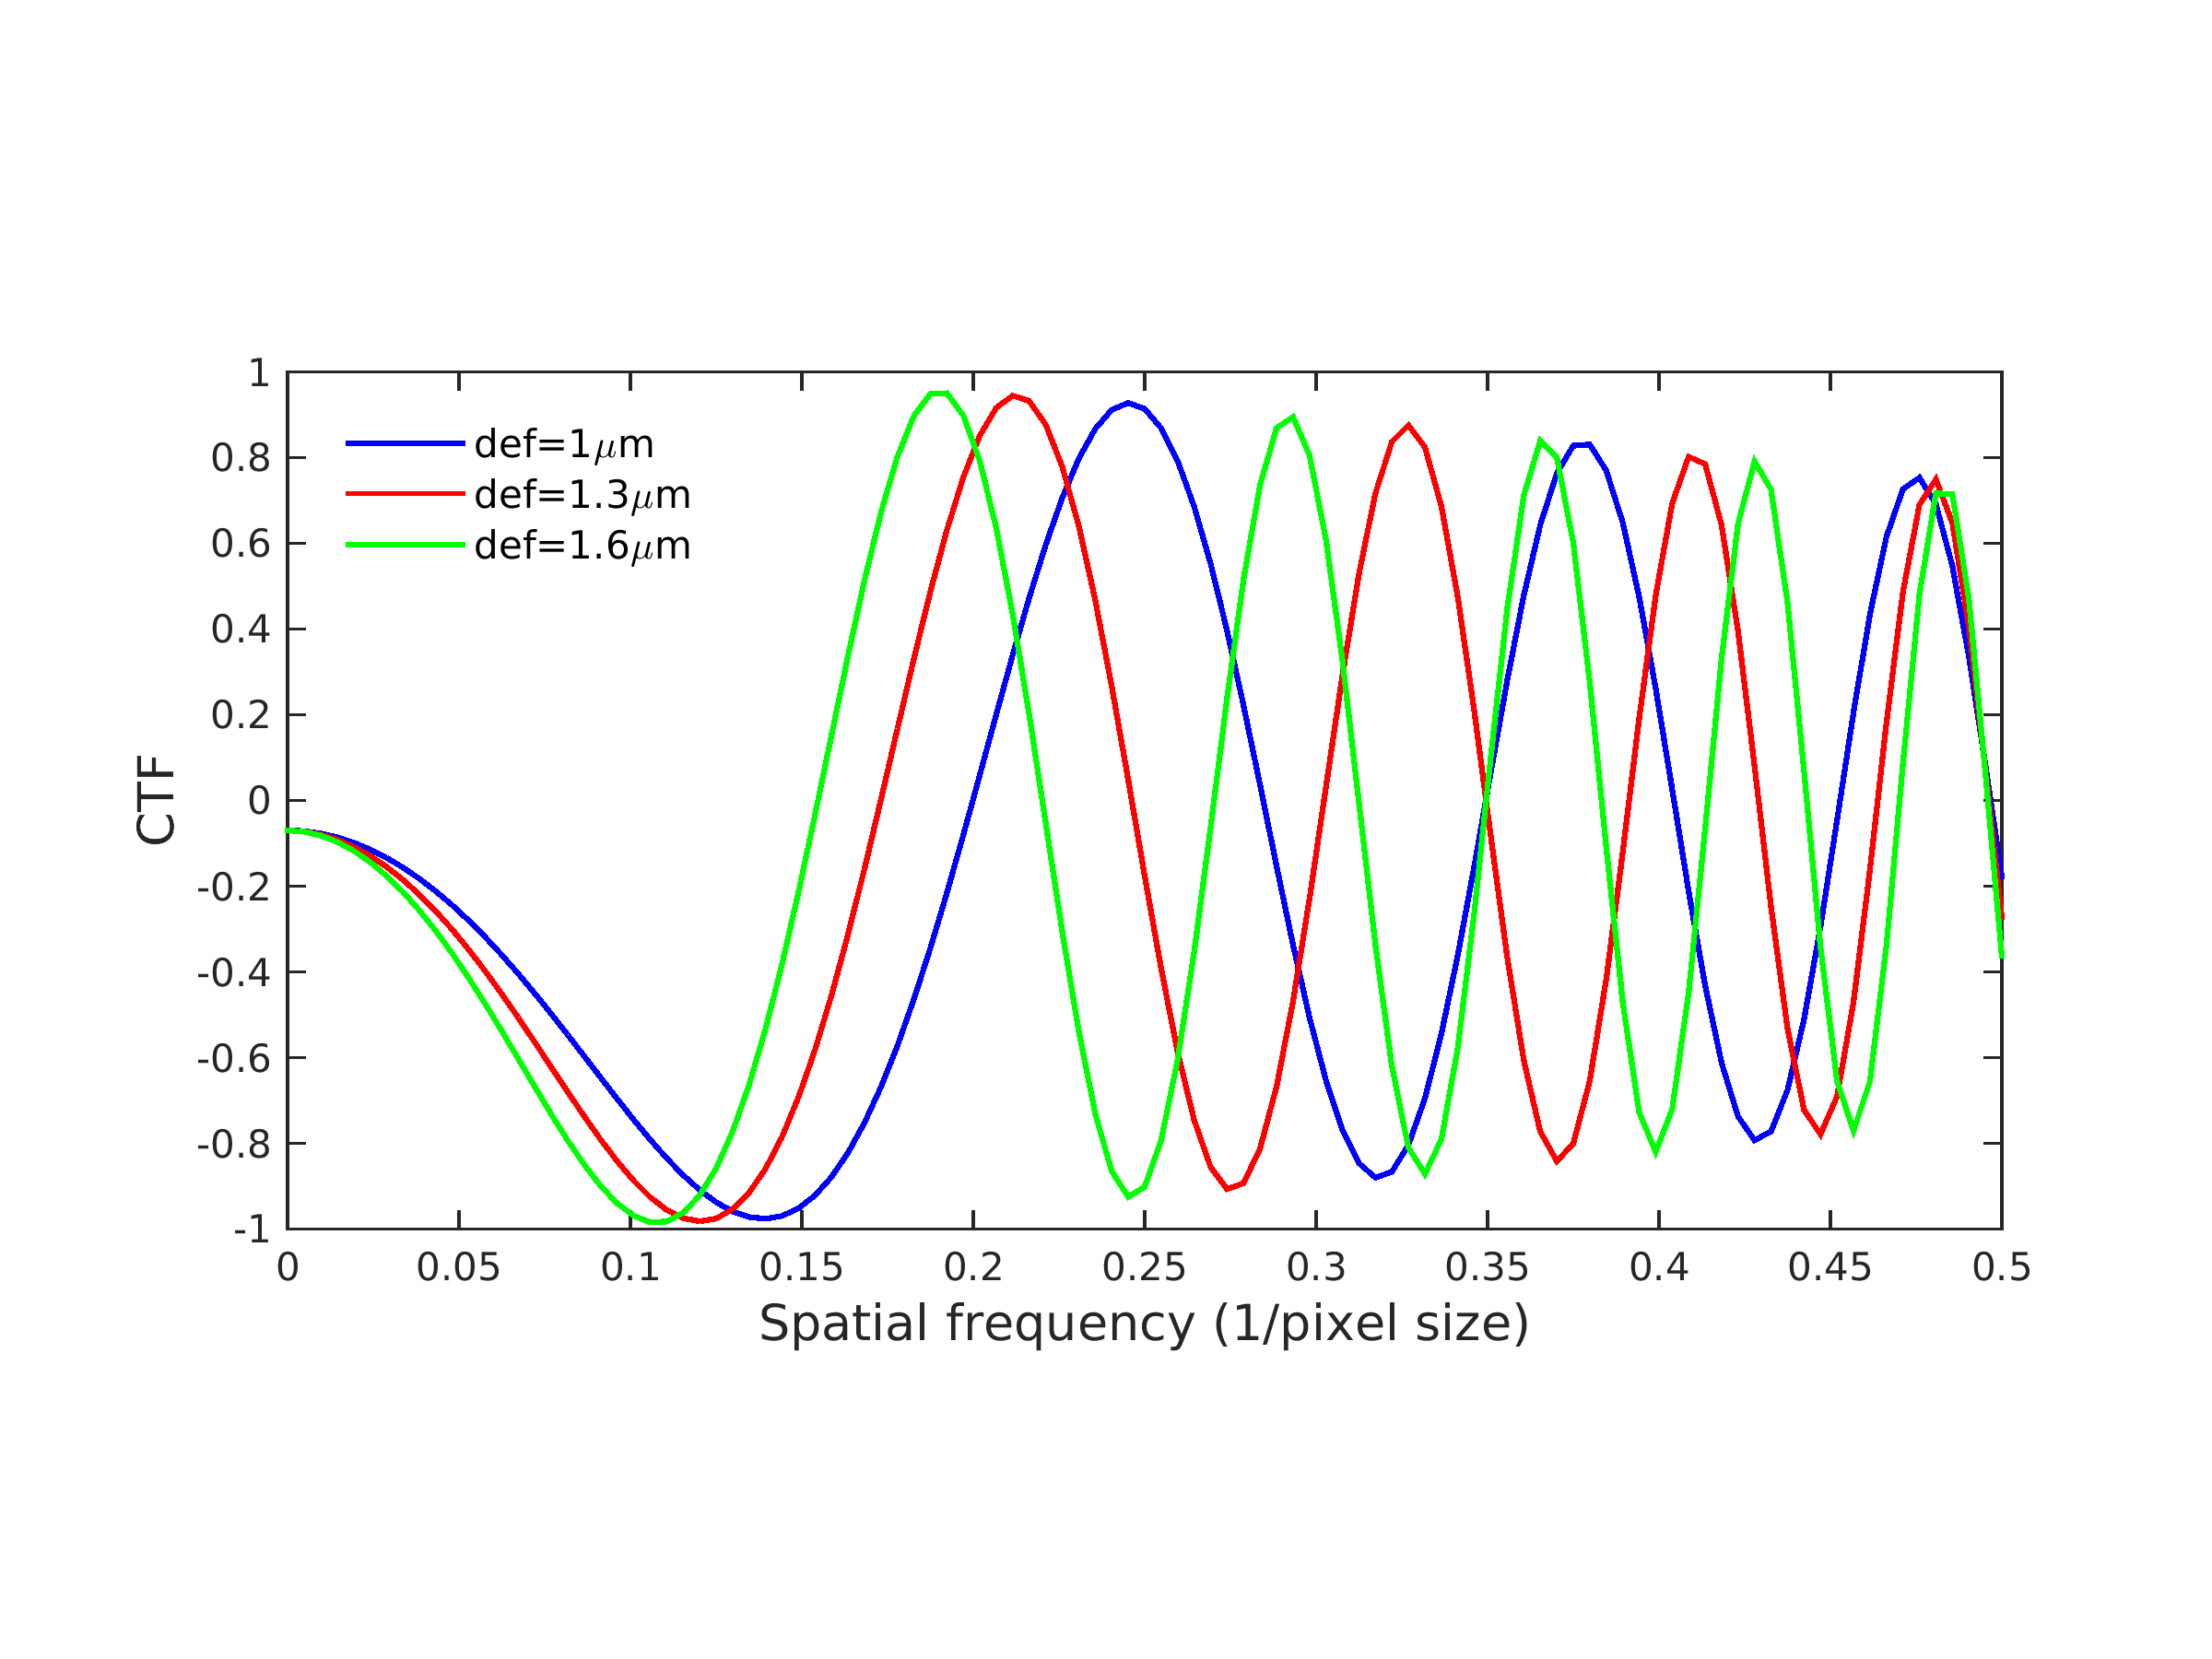
\includegraphics[scale=0.45]{figures/ctfeg_fig.png}
\end{figure}
\vspace{-12mm}
\begin{itemize}[]
\item Suppresses/loses information and inverts contrast
\item Not invertible (zero crossings)
\item Information lost from one defocus group could be recovered from another.
\end{itemize}
\end{frame}


\begin{frame}<beamer>
\setbeamercovered{transparent}
\frametitle{Current Image Restoration Techniques}
\begin{itemize}[]
 \item \textbf{Phase flipping + steerable PCA (sPCA)}: 
  \begin{itemize}
  \item  Flip sign of the Fourier
coefficients at frequencies for which the CTF is negative
   \item Preserves noise statistics
   \item Data adaptive basis: eigenvectors of the sample covariance matrix
   \item Phase flipping corrects only phases
  \end{itemize}
 \item \textbf{Traditional Wiener Filtering (TWF)}:
 \begin{itemize}
  \item  Corrects both phases and amplitudes
  \item Requires prior estimation of the spectral signal to
 noise ratio (SSNR)
  \item  Cannot restore information at zero crossings of the CTF
  \item Not in a data adaptive basis (restricted to Fourier basis)
 \end{itemize}
\end{itemize}
\end{frame}

\begin{frame}<beamer>
\setbeamercovered{transparent}
\frametitle{Covariance Wiener Filtering (CWF)}
\begin{itemize}[]
 \item Estimate the CTF-corrected covariance matrix of the
underlying clean 2D projection images
\item Wiener filtering to solve the image restoration deconvolution problem
\item No averaging, act on each image separately
\item CTF correction and denoising in a single step
\end{itemize}
\end{frame}

\begin{frame}<beamer>
\frametitle{Covariance Wiener Filtering (CWF)}
\begin{table}[h!]
\small
  \centering
  \caption{Comparison of CTF Correction/Denoising Methods}
  \begin{tabular}{cccc}
    \toprule
    Property & Phaseflip + sPCA & TWF & \alert{CWF}\\
    \midrule
    Applicable at preliminary stage & \cmark  & \cmark  & \cmark \\
    Data dependent basis & \cmark  &  \xmark & \cmark \\
    Correct both phases and amplitudes & \xmark  &  \cmark & \cmark \\
    CTF corrected covariance estimate & \textcolor{black}{\ding{51}}{\small\textcolor{black}{\kern-0.7em\ding{55}}}  &  \xmark & \cmark \\
 \bottomrule
  \end{tabular}
\end{table}
\end{frame}

\begin{frame}<beamer>
\frametitle{The Model: Real space}
Linear, weak phase approximation\\

\begin{equation*}
 y_i = a_i \ast x_i + \epsilon_i, \quad i=1,2,\ldots,n
\label{eqn:model}
\end{equation*}

$n$: number of images\\
$\ast$: convolution operation\\
$y_i$: noisy, CTF filtered $i$'th image in real space\\
$x_i$: underlying clean projection image in real space\\
$a_{i}$: the point spread function of the microscope\\
$\epsilon_i$: additive Gaussian noise that corrupts the image
\end{frame}

\begin{frame}<beamer>
\frametitle{The Model: Fourier space}

\begin{equation*}
 Y_i = A_i X_i + \xi_i, \quad i=1,2,\ldots,n
\label{eqn:model_f}
\end{equation*}

\begin{itemize}
\item $A_i$: diagonal operator (CTF)
\item $X_1,\dots,X_n$: vectors in $\mathbb{C}^p$, ($p$ is the number of pixels)
\item i.i.d. samples from a distribution with mean $\mathbb{E}[\textbf{X}]=\mu$
and covariance $\Sigma=\mathbb{E}[(\textbf{X}-\mu)(\textbf{X}-\mu)^T]$
\end{itemize}

\textbf{{``All models are wrong but some are useful" - George Box}}
\end{frame}

\begin{frame}<beamer>
\frametitle{The Model}
\begin{equation*}
\mathbb{E}[\textbf{Y}_i]=A_i \mathbb{E}[\textbf{X}_i], \quad i=1,2,\ldots,n.
\label{eqn:exp_y}
\end{equation*}

\begin{equation*}
\begin{aligned}
\mathbb{E}[(\textbf{Y}_i-\mathbb{E}[\textbf{Y}_i])(\textbf{Y}_i-\mathbb{E}[\textbf{Y}_i])^T] 
&= \mathbb{E} [A_i(\textbf{X}_i-\mu)(\textbf{X}_i-\mu)^T A_i^T] + \sigma^2I \\
&=  A_i \Sigma A_i^T + \sigma^2I .
\end{aligned}
\label{eqn:expectation_eq}
\end{equation*}

Relates the second order statistics of the noisy images with the 
population covariance $\Sigma$ of the clean images
\end{frame}


%%%%%

\begin{frame}<beamer>
\frametitle{Mean Estimation}

\begin{equation*}
 \hat\mu = \argmin{\mu} \sum_{i=1}^n||(Y_i-A_i\mu)||_2^2 + \lambda||\mu||_2^2
\end{equation*}

% % 
\begin{equation*}
 \hat\mu = (\sum_{i=1}^n A_i^T A_i + \lambda I)^{-1}(\sum_{i=1}^n 
A_i^T Y_i).
\label{eq:ls_mean_sol}
\end{equation*}
\end{frame}


\begin{frame}<beamer>
\frametitle{Covariance Estimation}
\begin{equation*}
\begin{aligned}
\hat\Sigma 
&= \argmin{\Sigma} \sum_{i=1}^n || (Y_i - \mathbb{E}[\textbf{Y}_i]) (Y_i - \mathbb{E}[\textbf{Y}_i])^T
- (A_i \Sigma A_i^T + \sigma^2 I)||_F^2 \\
&= \argmin{\Sigma} \sum_{i=1}^n || A_i\Sigma A_i^T + \sigma^2 I - C_i  ||_F^2 
\end{aligned}
\label{eqn:ls1}
\end{equation*}
where $C_i=(Y_i - A_i \mu) (Y_i - A_i \mu)^T$ and $||.||_F$ is the Frobenius matrix norm. 
\end{frame}


\begin{frame}<beamer>
\frametitle{Solving using Conjugate Gradient}
System of linear equations for the elements of the matrix $\hat \Sigma$

\begin{equation*}
\begin{aligned}
\sum_{i=1}^n  A_i^T  A_i \hat \Sigma A_i^T A_i
&= \sum_{i=1}^n A_i^T C_i A_i - \sum_{i=1}^n \sigma^2 A_i^T A_i 
\end{aligned}
\label{eqn:normal_white}
\end{equation*}
\frametitle{Solving using Conjugate Gradient}
\begin{equation*}
\begin{aligned}
L(\hat\Sigma) 
&=  B 
\label{eqn:cg}
\end{aligned}
\end{equation*}
where $L:\mathbb{R}^{p\times p} \to \mathbb{R}^{p\times p}$ is the linear operator acting on $\hat{\Sigma}$.

\begin{itemize}
 \item Direct inversion of this linear system is slow for large image sizes
 \item Applying $L$ only involves matrix multiplications: fast!
 \item Conjugate gradient 
\end{itemize}

\end{frame}


\begin{frame}<beamer>
\frametitle{Eigenvalue Thresholding}
\setbeamercovered{transparent}
\begin{itemize}[]
 \item  $L(\hat{\Sigma})$ is a PSD matrix whenever $\hat{\Sigma}$ is PSD (as 
a sum of PSD matrices)
\item  $B$ may not necessarily be PSD due to finite 
sample fluctuations 
\item  Project $B$ onto the cone of PSD matrices
\item  Compute the spectral 
decomposition of $B$ and set all negative eigenvalues to 0  (eigenvalue thresholding)
\end{itemize}
\end{frame}

\begin{frame}<beamer>
\frametitle{High Dimensional PCA}
\setbeamercovered{transparent}
\begin{itemize}[]
\item $n \asymp p$ regime: sample covariance not a good approximation to the population covariance * \blfootnote{* Johnstone (2001)}
\item Mar\v{c}enko-Pastur distribution
\end{itemize}
\begin{columns}
\column{0.5\linewidth}
\begin{figure}
\centering
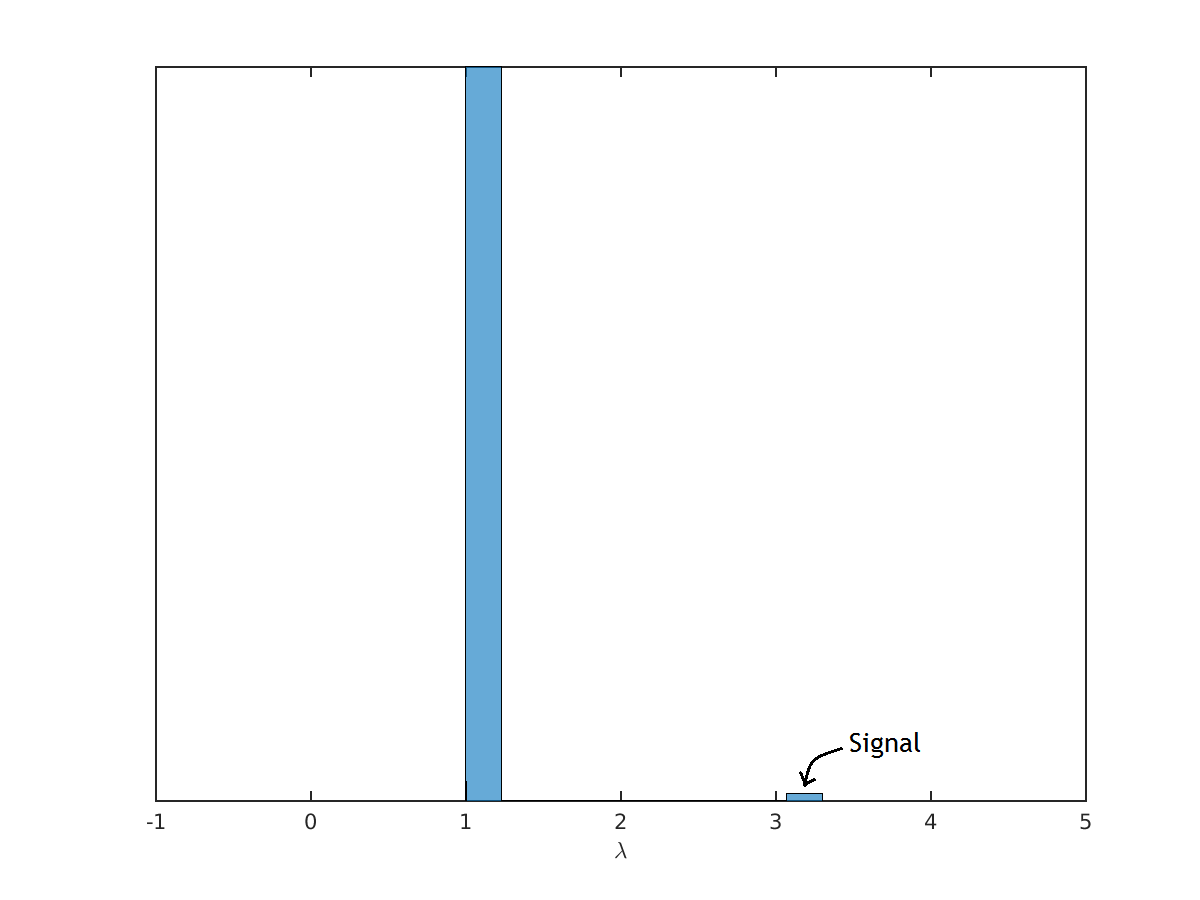
\includegraphics[width=1\linewidth]{figures/mpplot_clt.png}
\caption{$n \gg p$}
\end{figure}
\column{0.5\linewidth} 
\begin{figure}
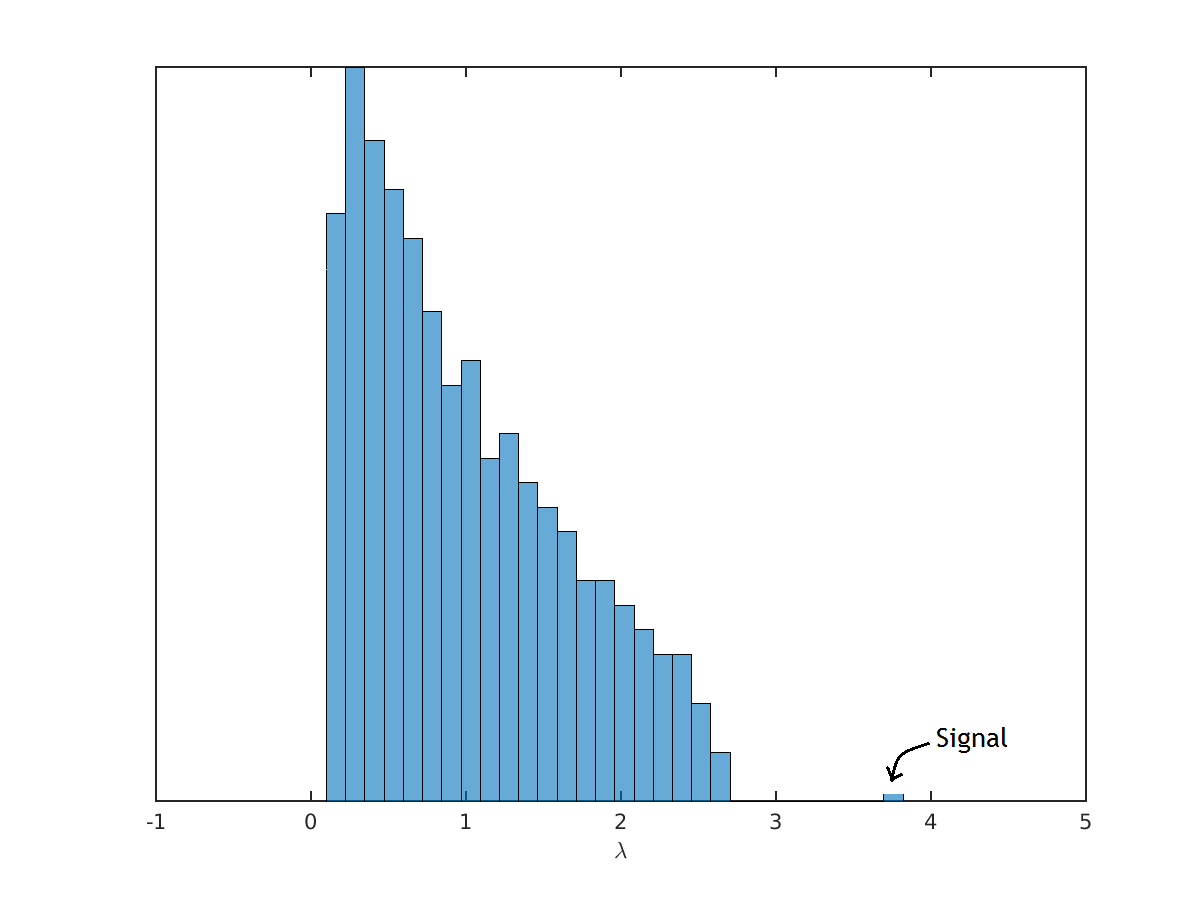
\includegraphics[width=1\linewidth]{figures/mpplot_high.png}
\caption{$n \asymp p$}
\label{fig:shrinkage}
\end{figure}
\end{columns}
\end{frame}

\begin{frame}<beamer>
\frametitle{Eigenvalue Shrinkage: Spiked Covariance Model}
\setbeamercovered{transparent}
\begin{itemize}[]
\item Select eigenvalues corresponding to the signal* \blfootnote{* Kritchman and Nadler (2008)}
\item High dimensional $n \asymp p$ regime: eigenvalue 
shrinkage procedure**\blfootnote{** Donoho et al.(2013)} 
\end{itemize}
\begin{columns}
\column{0.5\linewidth}
\begin{figure}
\centering
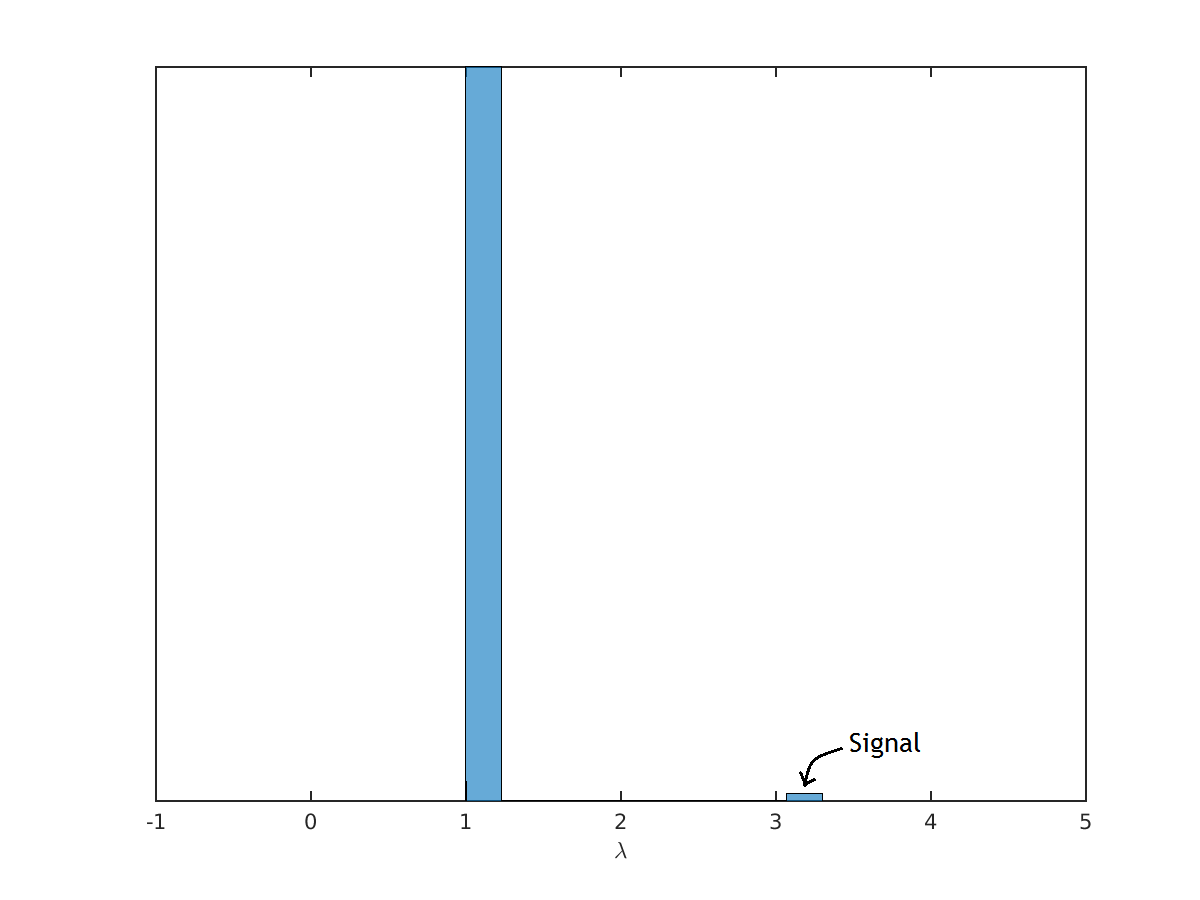
\includegraphics[width=1\linewidth]{figures/mpplot_clt.png}
\caption{$n \gg p$}
\end{figure}
\column{0.5\linewidth} 
\begin{figure}
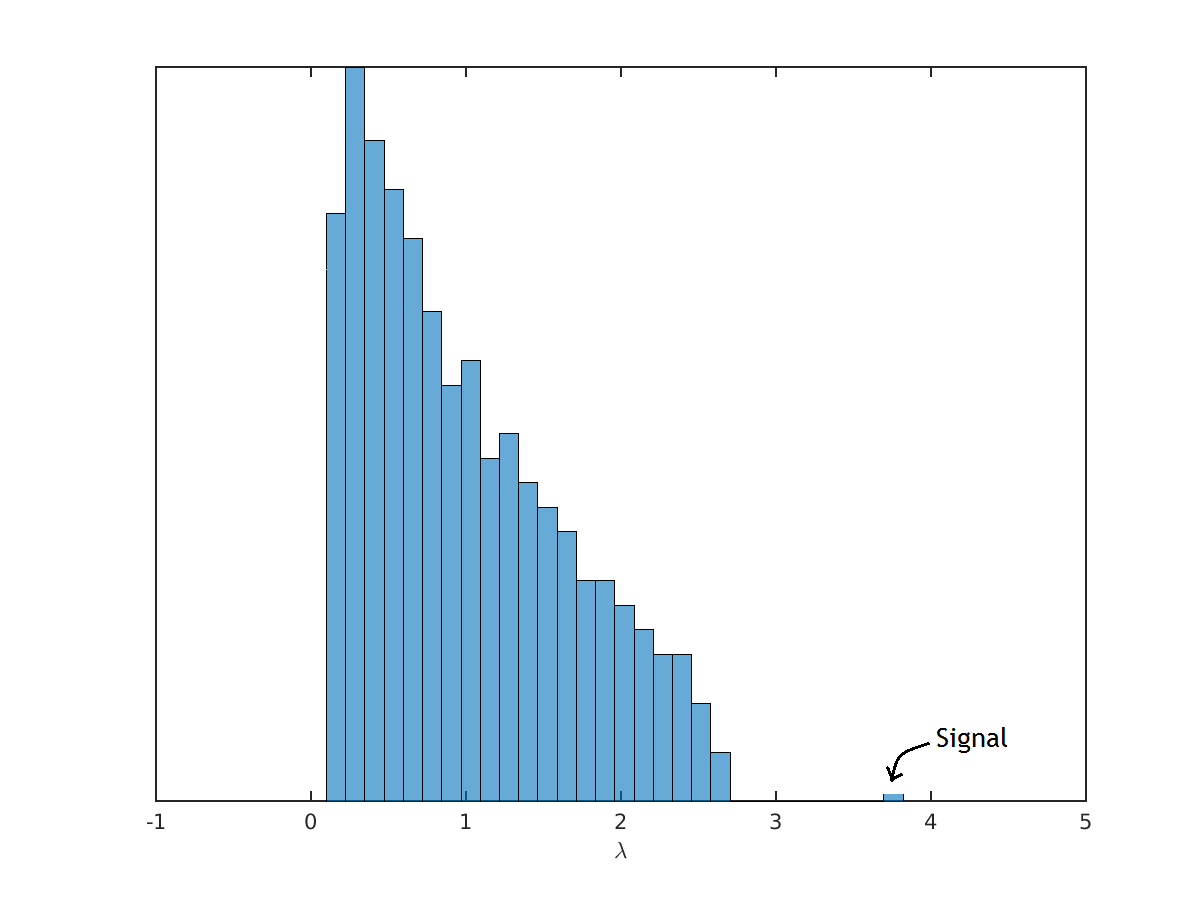
\includegraphics[width=1\linewidth]{figures/mpplot_high.png}
\caption{$n \asymp p$}
\label{fig:shrinkage}
\end{figure}
\end{columns}
\end{frame}


\begin{frame}<beamer>
\frametitle{Deconvolution by Wiener Filtering}

\begin{itemize}
\item White noise: estimate $X_i$ as
\begin{equation*}
\hat X_i = (I-H_iA_{i})\hat\mu + H_iY_i 
\end{equation*}
where $H_i = \hat \Sigma A_{i}^T ( A_{i} \hat \Sigma A_{i}^T + \sigma^2 
I)^{-1} $ is the linear Wiener filter  
\item Colored noise: estimate $X_i$ as
\begin{equation*}
\hat X_i = (I-H_iWA_{i})\hat\mu + H_iY_i 
\end{equation*}
with $H_i = \hat \Sigma A_{i}^T W^T (W A_{i} \hat \Sigma A_{i}^T W^T 
+ \sigma^2 I)^{-1}$
\end{itemize}
\end{frame}


\begin{frame}<beamer>
\setbeamercovered{transparent}
\frametitle{Fourier-Bessel Steerable Basis }
\begin{figure}
\centering
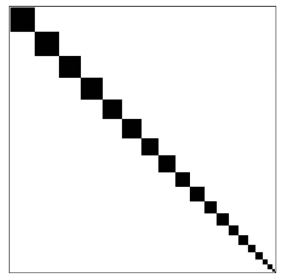
\includegraphics[width=0.2\linewidth]{figures/blockcov.png}
\caption{Z. Zhao and A. Singer (2013)}
\end{figure}
\begin{itemize}[]
\item Population covariance matrix $\Sigma$ invariant under in-plane 
rotation of projection images
\item Block diagonal in any steerable basis in which the 
basis elements are outer products of radial functions and angular Fourier modes
\item \textbf{Nearly unitary transformation: noise statistics preserved}
\item \textbf{Fast computation} for each block separately
\end{itemize}
\end{frame}

\begin{frame}<beamer>
\frametitle{Computational Complexity}
$O(TDL^4 + nL^3)$, where $T$ is the number of conjugate gradient iterations
\begin{itemize}
\item $D$ defocus groups
\item Images of size $L \times L$
\item \textit{n} images
\end{itemize}
\end{frame}


\begin{frame}<beamer>
\frametitle{Computational Complexity: Timings}
$n$ images of size $L \times L$\\
UNIX environment with 60 cores,
running at 2.3 GHz, with total RAM of 1.5TB


\begin{table}[t]
  \centering
  \caption{Timing in seconds}
  \begin{tabular}{ccccc}
    \toprule
    Dataset & $L$ & $n$ & Basis coeffs  & CWF \\
    \midrule
    TRPV1 & 256 & 35645 & 312s & 574s \\
    80s & 360 & 30000 &  731s & 385s \\
    IP3R1  & 256 & 37382 & 429s & 589s\\
    70s & 250 &  99979 & 1174s & 113s \\
 \bottomrule
  \end{tabular}
\end{table}
\end{frame}



\begin{frame}<beamer>
\frametitle{Relative error of estimated covariance}
\begin{figure}
\centering
\includegraphics[width=0.6\linewidth]{figures/cwf_shrinkage_compare.eps}
\caption{The estimator $\hat \Sigma$ can be shown to be consistent in the large sample limit
$n \to \infty$}
\label{fig:shrinkage}
\end{figure}
\end{frame}

\begin{frame}<beamer>
\frametitle{Simulations with white noise:  80S ribosome (EMDB-6454)}

\begin{figure}[]
\centering
\subfloat[SNR=$1$]{\begin{overpic}[width=0.35\linewidth]{figures/compare_ims_snr1by1_6454.eps}
\put(6,52){\tiny Clean}
\put(32,52){\tiny Noisy}
\put(55,52){\tiny TWF}
\put(80,52){\tiny CWF}
\put(-40,35){\tiny Defocus=$1\mu m$}
\put(-40,10){\tiny Defocus=$4\mu m$}
\end{overpic}%
}\quad
%\vspace{-0.5mm}
\subfloat[SNR=$1/20$]{\begin{overpic}[width=0.35\linewidth]{figures/compare_ims_snr1by20_6454.eps}%
%\put(5,40){Clean}
\end{overpic}%
\label{}}\\
%\vspace{-0.5mm}
\subfloat[SNR=$1/40$]{\begin{overpic}[width=0.35\linewidth]{figures/compare_ims_snr1by40_6454.eps}%
%\put(5,40){Clean}
\end{overpic}%
\label{}}\quad
%\vspace{-0.5mm}
\subfloat[SNR=$1/60$]{\begin{overpic}[width=0.35\linewidth]{figures/compare_ims_snr1by60_6454.eps}%
%\put(5,40){Clean}
\end{overpic}%
\label{}}

\label{fig:ims_6454}
\end{figure}

\end{frame}


\begin{frame}<beamer>
\frametitle{Outlier Detection}
\setbeamercovered{transparent}
\begin{itemize}[]
 \item  Current method: manual visual inspection after particle picking
\item CWF: automatic way to classify picked particles
\item Specimen particles at various depths in the ice layer: acquired
projection images can have different contrasts
\item 
\begin{equation*}
 Y_i = \alpha_i A_i X_i + \xi_i, \quad i=1,2,\ldots,n
\label{eqn:contrast}
\end{equation*}
\item Absorb $\alpha$ into $\textbf{X}$ and estimate $\alpha_i X_i$ 
\item  Outlier images typically have low contrast
after denoising: linear classifier
after CWF 
\end{itemize}
\end{frame}
\setcounter{subfigure}{0}
\begin{frame}<beamer>
\frametitle{Outlier Detection: 80S ribosome (EMDB-6454)}
SNR=1/20 
$\alpha \in [0.75,1.5]$
$10\%$ images are pure noise
\begin{figure}[]
\centering
\subfloat[]{\begin{overpic}[width=0.34\linewidth]{figures/raw_title.eps}%
\end{overpic}%
\label{fig:raw_outlier}}
\quad
\subfloat[]{\begin{overpic}[width=0.34\linewidth]{figures/den_title.eps}
\end{overpic}
\label{fig:den_outlier}} \\
\subfloat[]{\begin{overpic}[width=0.1\linewidth]{figures/mean_image.eps}%
\end{overpic}%
\label{fig:mean_image}}
\quad
\subfloat[]{\begin{overpic}[width=0.45\linewidth]{figures/top_eigim.eps}
\end{overpic}
\label{fig:eigenims}}
\end{figure}
\end{frame}


\begin{frame}<beamer>
\frametitle{Experimental data - 80S ribosome}

\begin{figure}[h]
\centering
{\begin{overpic}[width=0.5\textwidth]{figures/jsb_fig_80s.eps}%
\put(8,77){\tiny Raw}
\put(22,77){\tiny Closest projection}
\put(59,77){\tiny TWF}
\put(83,77){\tiny CWF}
\end{overpic}
\label{}}
\label{fig:real80s}
\end{figure}
%  FEI
\begin{itemize}
 \item FALCON II 4k$\times$4k direct electron detector\\
 \item 105247 motion corrected, picked particle images of 360$\times$360 pixels
\end{itemize}
\end{frame}


\begin{frame}<beamer>
\frametitle{Experimental data - TRPV1}
 
\begin{figure}[h]
\centering
{\begin{overpic}[width=0.5\textwidth]{figures/jsb_fig_tv.eps}%
\put(10,77){\tiny Raw}
\put(22,77){\tiny Closest projection}
\put(59,77){\tiny TWF}
\put(82,77){\tiny CWF}
\end{overpic}
\label{}}

\label{fig:trpv1}
\end{figure}
% 
\begin{itemize}
 \item K2 direct electron detector\\
 \item 35645 motion corrected, picked particle images of 256$\times$256 pixels
\end{itemize}
\end{frame}


\begin{frame}<beamer>
\frametitle{Experimental data -IP\textsubscript{3}R1}
\begin{figure}[h]
\centering
{\begin{overpic}[width=0.5\textwidth]{figures/jsb_fig_ip3.eps}%
\put(10,77){\tiny Raw}
\put(22,77){\tiny Closest projection}
\put(57,77){\tiny TWF}
\put(83,77){\tiny CWF}
\end{overpic}
\label{}}
\label{fig:ip3}
\begin{itemize}
 \item Gatan 4k$\times$4k CCD\\
 \item 37382 picked particle images of 256$\times$256 pixels
\end{itemize}
\end{figure}
\end{frame}

\begin{frame}<beamer>
\frametitle{Experimental data - 70S ribosome}
\begin{figure}[h]
\centering
{\begin{overpic}[width=0.5\textwidth]{figures/jsb_fig_70s.eps}%
\put(10,77){\tiny Raw}
\put(22,77){\tiny Closest projection}
\put(58,77){\tiny TWF}
\put(82,77){\tiny CWF}
\end{overpic}
\label{}}
\label{fig:real70s}
\end{figure}
\begin{itemize}
 \item TVIPS TEMCAM-F415 (4k x 4k) CCD\\
 \item 216517 picked particle images of 250$\times$250 pixels
\end{itemize}
\end{frame}
%
%\begin{frame}<beamer>
%\frametitle{Application: Mahalanobis Affinity}
%Mahalanobis affinity or likelihood for the underlying clean images $x_i$ and $x_j$ to originate from the same viewing direction \blfootnote{TB, Z. Zhao and A. Singer (2017)}
%\begin{align}
%&\Pr(||X_{ij}||_{p} < \epsilon|Y_i=y_i,Y_j=y_j)   \nonumber
%%										 
%\end{align}
%\begin{equation*}
%= \frac{\epsilon^d \text{Vol}(B_p(0,1)) }{(2 \pi)^{\frac{d}{2}} |L_i + L_j|^{\frac{1}{2}}} \exp\{-\frac{1}{2}\alpha_{ij}^T(L_i+L_j)^{-1}\alpha_{ij}\} +  \mathcal{O}(\epsilon^{d+1})   \nonumber
%\label{eqn:metr}
%\end{equation*}
%\end{frame}
%
%\begin{frame}<beamer>
%\setbeamercovered{transparent}
%\frametitle{New Class Averaging Pipeline}
%\begin{figure}[h]
%\centering
%{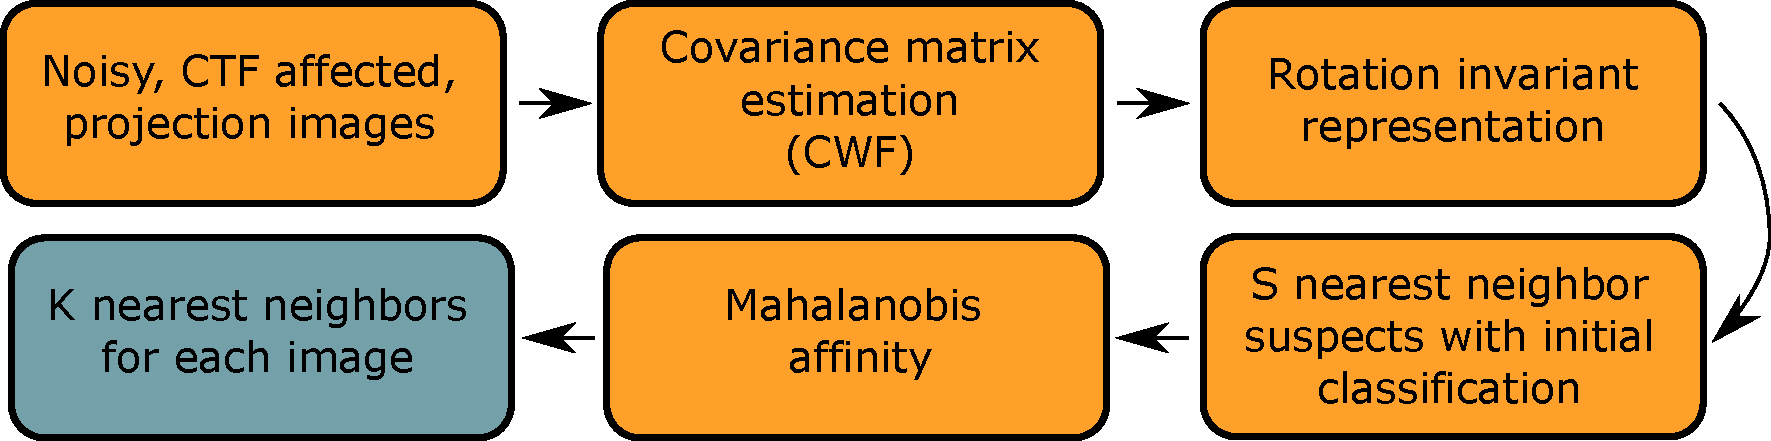
\includegraphics[scale=0.4]{figures/pipeline.pdf}}\\
%\label{fig:rawims}
%\end{figure}
%\end{frame}
%
%
%\begin{frame}<beamer>
%\frametitle{Class Averages}
%\begin{figure}[!htbp]
%\begin{center}
%\begin{tabular}{c}
%%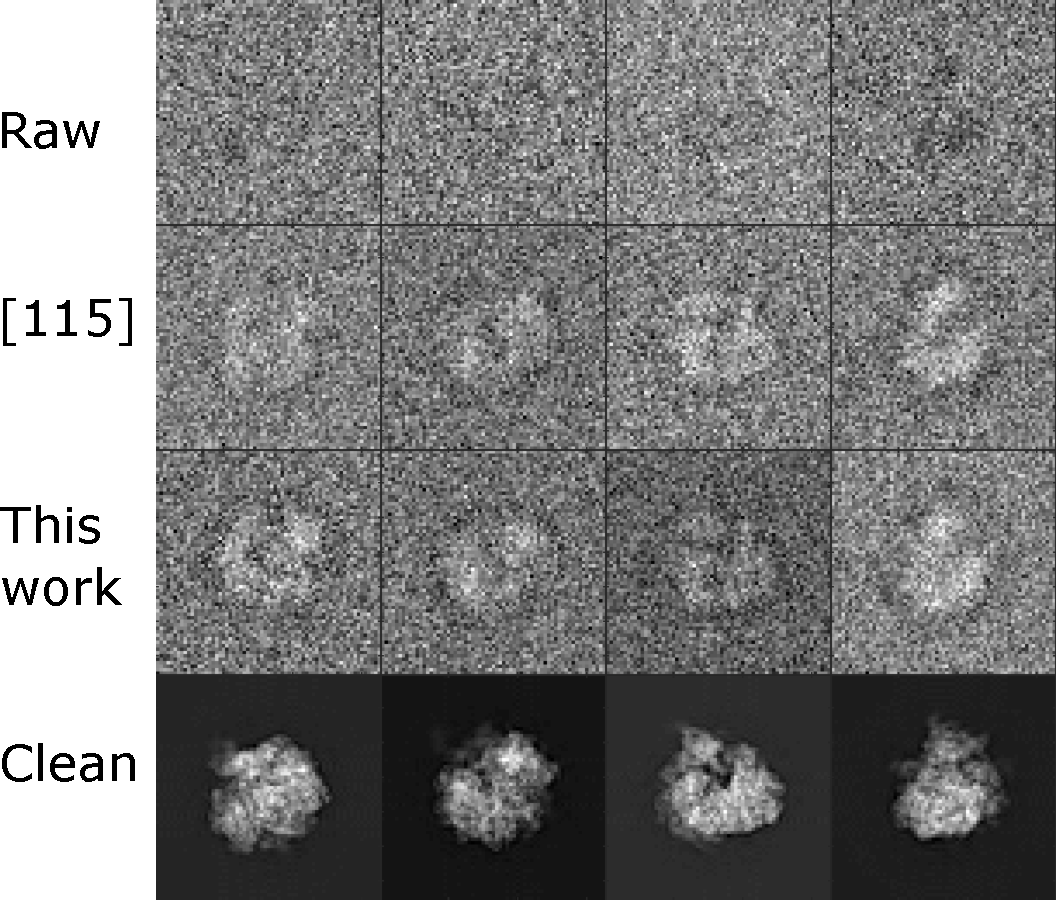
\includegraphics[width=.48 \columnwidth]{figures/classavg_mah_K10_2.pdf}\\
%%(a)\\
%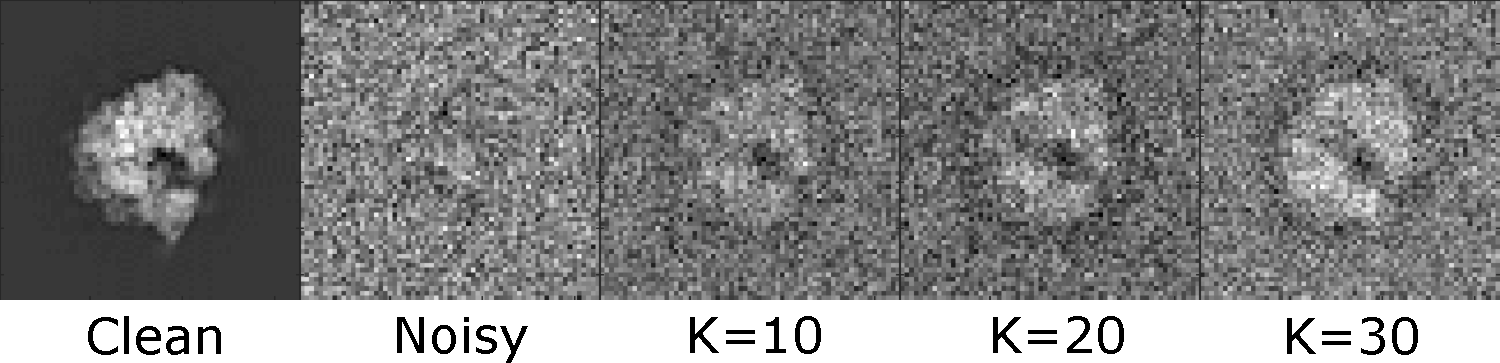
\includegraphics[width=.8 \columnwidth]{figures/classavg_fig3.pdf}\\
%%(b)
%\end{tabular}
%\end{center}
%\caption{ Class averages with the improved algorithm using the anisotropic affinity, using $K=10,\ 20,\ 30$.  \blfootnote{TB, Z. Zhao and A. Singer (2017)}}
%\end{figure}
%\end{frame}
%
%\begin{frame}<beamer>
%\frametitle{Improved Nearest Neighbor Detection}
%\begin{figure}
%\begin{center}
%\begin{tabular}{cc}
%%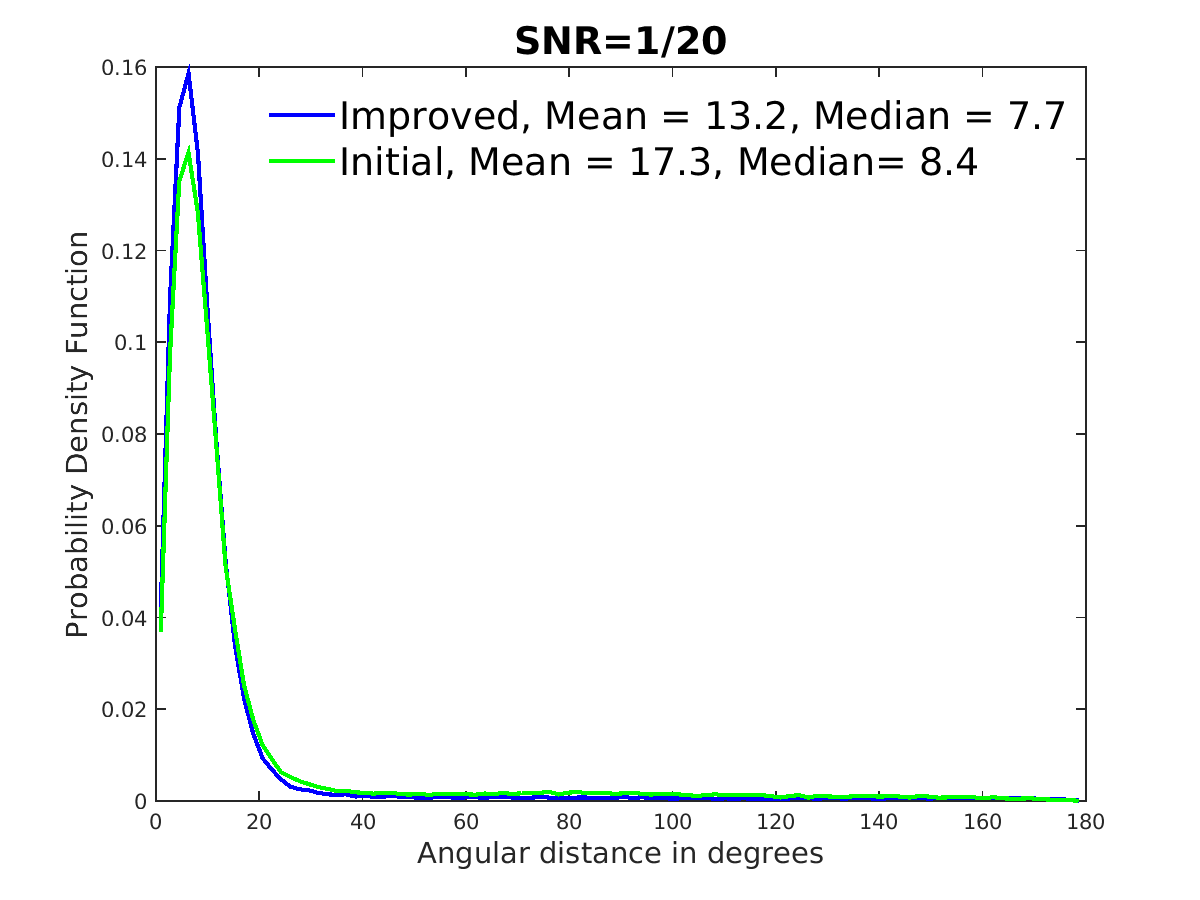
\includegraphics[width=.35\columnwidth]{figures/fighist_snr1by20.png} & 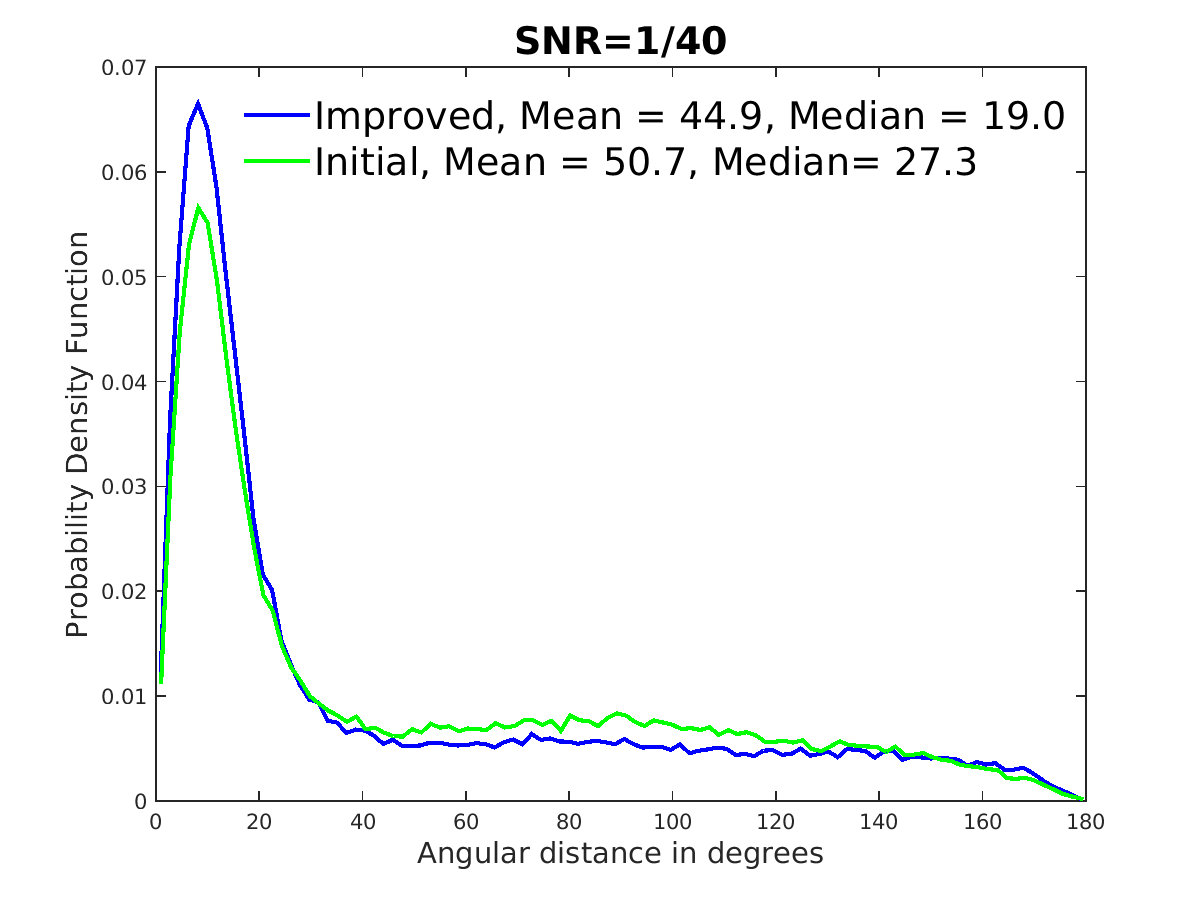
\includegraphics[width=.35\columnwidth]{figures/fighist_snr1by40.png} \\
%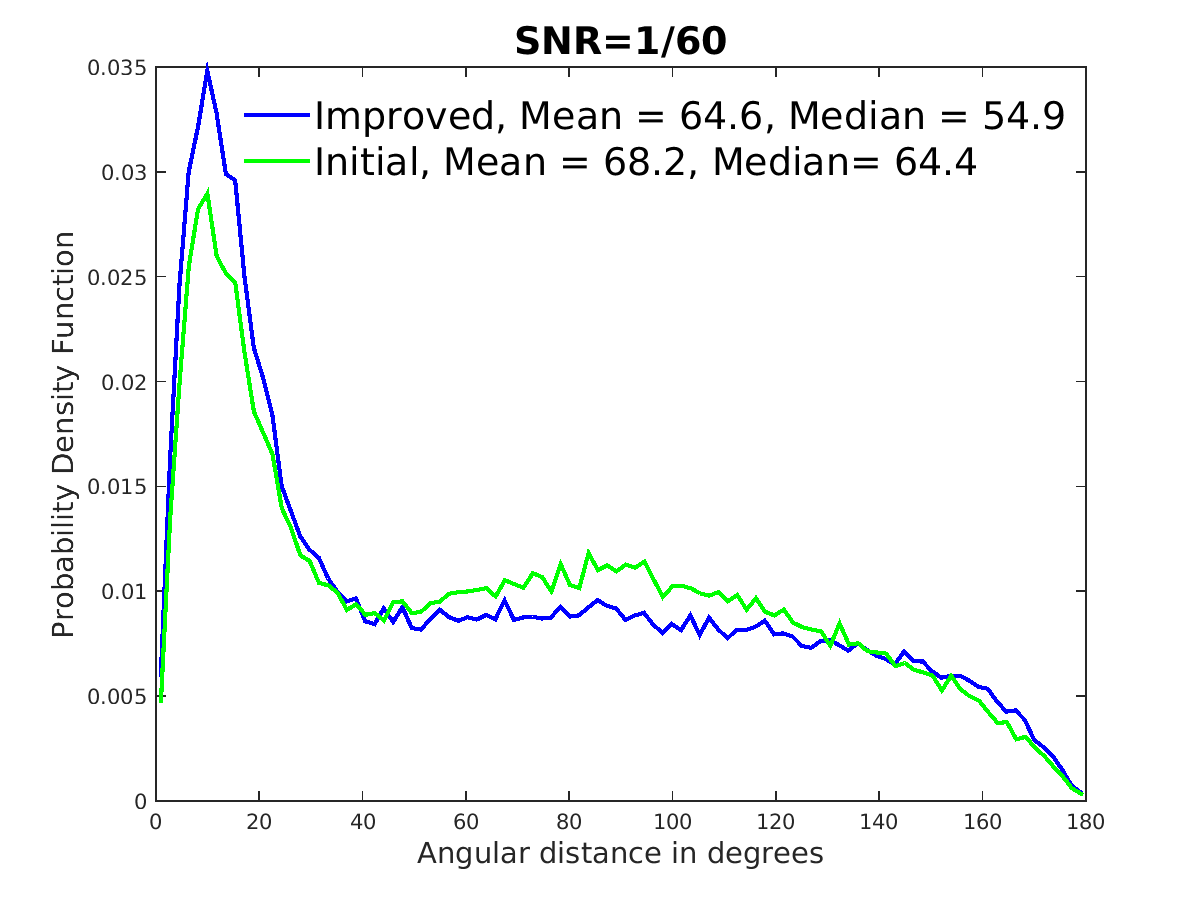
\includegraphics[width=.49\columnwidth]{figures/fighist_snr1by60.png} & 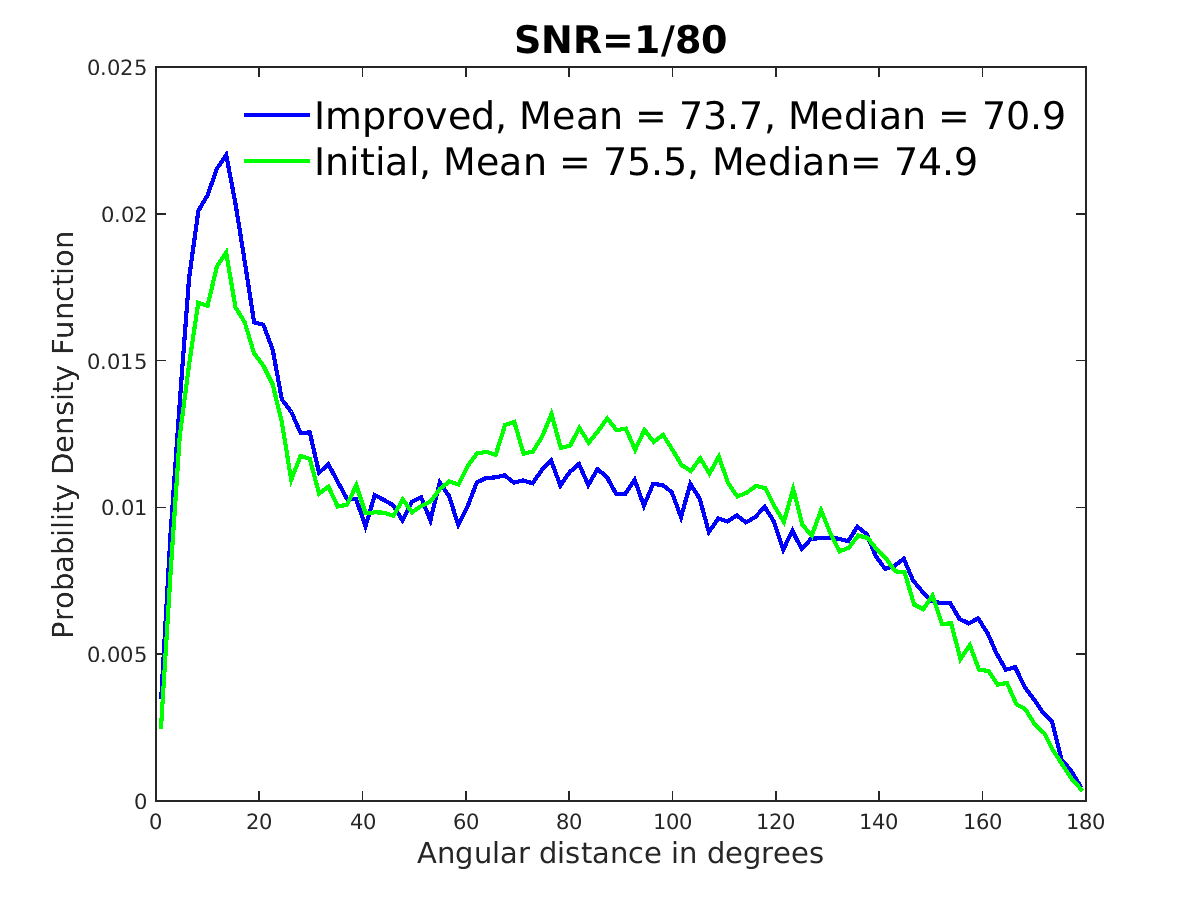
\includegraphics[width=.49\columnwidth]{figures/fighist_snr1by80.png}
%\end{tabular}
%\end{center}
%\end{figure}
%Improved nearest neighbor detection using Mahalanobis affinity\blfootnote{TB, Z. Zhao and A. Singer (2017)}
%\end{frame}


\section{Part 2: 3D Homology Modeling}

\begin{frame}<beamer>
\setbeamercovered{transparent}
\frametitle{Existing Methods: Ab Initio Modeling}
\begin{columns}
\column{0.3\linewidth}
\begin{figure}
\centering
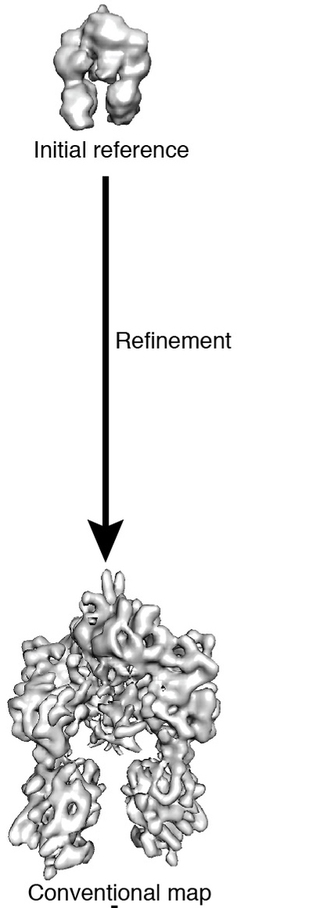
\includegraphics[width=.7 \columnwidth]{figures/refinement.png}
\end{figure}
\column{0.7\linewidth} 
\begin{itemize}
 \item \textbf{Random conical tilt} (Radermacher et al.): tilting to acquire two sets of micrographs
 \item \textbf{Method of moments} (Goncharov et al., Salzman, et al.): sensitive to errors in data
 \item \textbf{Common lines approach} (Singer et al.): needs class averaging
\end{itemize}
\end{columns}
\end{frame}

\begin{frame}<beamer>
\begin{figure}
\centering
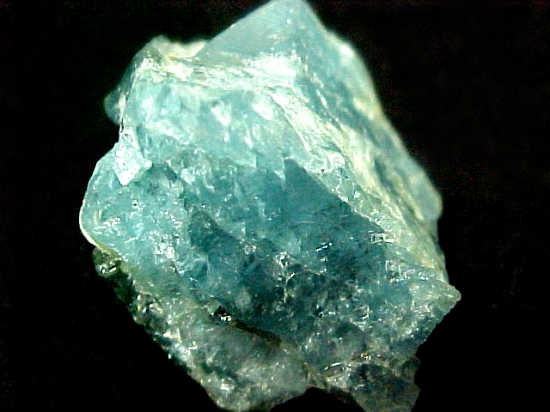
\includegraphics[width=.25 \columnwidth]{figures/beryl.jpg} \quad 
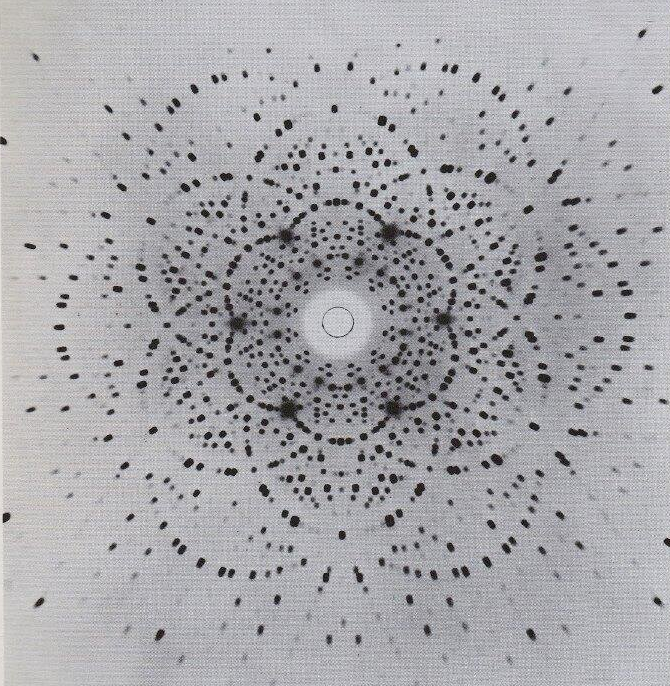
\includegraphics[scale=0.15]{figures/diffpattern.png}
\caption{X-ray diffraction pattern of Beryl}
\end{figure}
\frametitle{Motivation: Molecular Replacement (MR)}
\begin{itemize}
\item \textbf{Missing phase problem} in X-ray crystallography
\item Use previously solved homologous structure
\item Fourier magnitudes from unknown structure, phases from homologous structure
\end{itemize}
\end{frame}


\begin{frame}<beamer>
\frametitle{A Tail of Two Cats}
\begin{itemize}

\item Expansion coefficients $\bB$: known structure, $\bA$: unknown structure, $2\hat{\bA}_{\text{LS}}$ estimate for unknown structure
\item $2\hat{\bA}_{\text{LS}}-\bB$ for $\bA\in\mathbb{C}^{1\times 1}$ is an unbiased estimator (\textbf{`Twicing'} for magnitude correction) \blfootnote{J. Tukey (1977), P. Main (1979), K. Cowtan (2014)}
\end{itemize}
\begin{figure}[]
\centering
\begin{tabular}{cc}
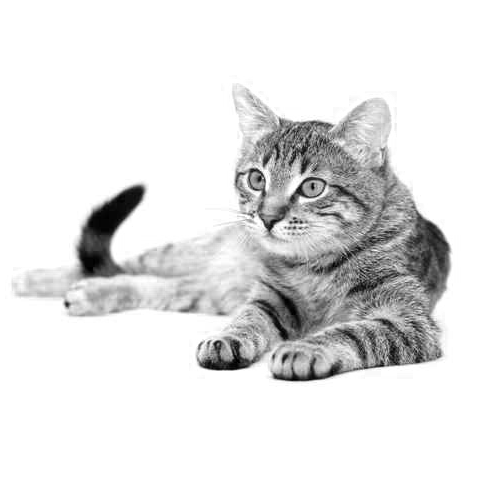
\includegraphics[width=0.15\linewidth]{figures/cat.png}
&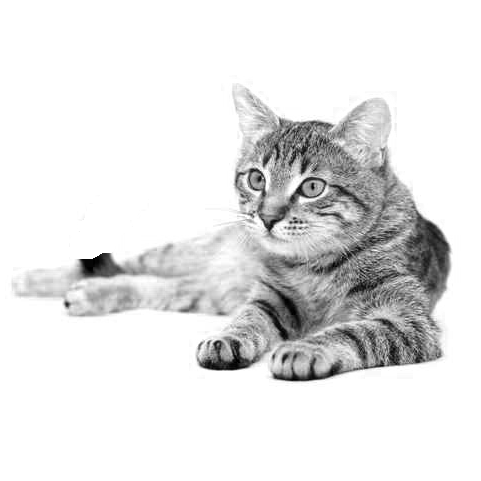
\includegraphics[width=0.15\linewidth]{figures/cat_tail.png}\\
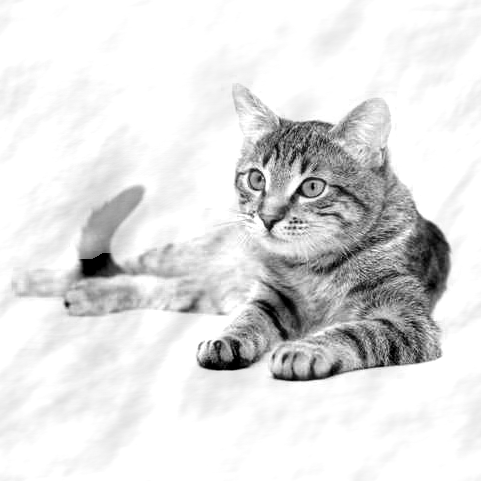
\includegraphics[width=0.15\linewidth]{figures/cat_t1.png}
&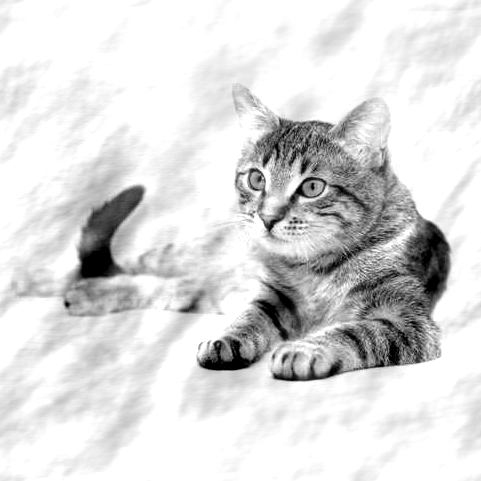
\includegraphics[width=0.15\linewidth]{figures/cat_t2.png}\\
\end{tabular}
\label{fig:tail_cat}
\end{figure}
\end{frame}

\begin{frame}<beamer>
\frametitle{New approach for homology modeling}
\begin{itemize}
\item Two new algorithms to predict structure \textbf{directly from raw images (no averaging)}
\item Use previously solved homologous structure 
\item Use Kam's autocorrelation analysis \blfootnote{Z. Kam (1980, 1985)}
\end{itemize}
\end{frame}


\begin{frame}<beamer>
\frametitle{Kam's Autocorrelation Analysis}
\begin{equation*}
\label{eq:Cl}
\bC_{{\bl}}= \bA_{\bl} \bA_{\bl}^*  \quad l=0,1,\ldots
\end{equation*}

\begin{itemize}
\item $\bC_{\bl}$: autocorrelation matrix over $SO(3)$ (\alert{``magnitude''})
\item $\bA_{\bl}$: Expansion coefficients of 3D Fourier volume
\item $\bC_{\bl}$ can be computed from the covariance matrix $\Sigma$ of the 2D projection images \blfootnote{Z. Kam (1980, 1985)}
\item Requirement: Uniformly distributed viewing angles over the sphere
\end{itemize}
\end{frame}


\begin{frame}<beamer>
\frametitle{Outline of Our Approach}
\begin{equation*}
\label{eq:Cl}
\bC_{{\bl}}= \bA_{\bl} \bA_{\bl}^*  \quad l=0,1,\ldots
\end{equation*}

\begin{itemize}

\item $\bC_{\bl}$ can be computed from the covariance matrix $\Sigma$
\item Use estimated $\hat\Sigma$ from Covariance Wiener Filtering to compute $\bC_{\bl}$ (\alert{``magnitude''})
\item Determines $\bA_{\bl}$ upto an orthogonal matrix (\alert{``missing phase''})
\end{itemize}
\end{frame}

\begin{frame}<beamer>
\frametitle{Orthogonal Matrix Retrieval Problem \blfootnote{TB, T. Zhang, A. Singer (2015)}}
\begin{itemize}
\item $\Phi_A: \mathbb{R}^3 \rightarrow \mathbb{R}$: electron scattering 
density of the unknown structure.
\item $\mathcal{F}(\Phi_A) : \mathbb{R}^3 \to \mathbb{C}$: 3D Fourier transform
\end{itemize}


\begin{equation*}
\label{eq:phia_expansion_full}
\mathcal{F}(\Phi_A)(k,\theta,\varphi) = \sum_{l=0}^{\infty} \sum_{m=-l}^{l} 
A_{lm}(k)
Y_l^m
(\theta, \varphi) \nonumber
\end{equation*}
\begin{itemize}
\item $k$: radial frequency
\item $Y_l^m$: real spherical harmonics
\end{itemize}
\end{frame}

\begin{frame}<beamer>
\frametitle{Kam's Autocorrelation Analysis}
\begin{equation*}
\label{eq:phia_expansion_full}
\mathcal{F}(\Phi_A)(k,\theta,\varphi) = \sum_{l=0}^{\infty} \sum_{m=-l}^{l} 
A_{lm}(k)
Y_l^m
(\theta, \varphi) \nonumber
\end{equation*}

\begin{equation*}
\label{eq:Cl}
C_{{l}}(k_1,k_2) = \sum_{m=-l}^l A_{lm}(k_1)\overline{A_{lm}(k_2)}, \quad 
l=0,1,\ldots \nonumber
\end{equation*}

\begin{itemize}
\item $\bC_{\bl}$: autocorrelation matrix over $SO(3)$
\item $\bC_{\bl}$ can be estimated from the covariance matrix $\Sigma$ of the 2D projection images \blfootnote{Z. Kam (1980)}
\item Requirement: Uniformly distributed viewing angles over the sphere
\end{itemize}
\end{frame}

\begin{frame}<beamer>
\frametitle{Resolution Limit}
\begin{itemize}
\item Finite pixel grid: Nyquist criterion
\end{itemize}
\begin{equation*}\label{eq:phia_expansion}
\mathcal{F}(\Phi_A)(k,\theta,\varphi) = \sum_{l=0}^{L} \sum_{m=-l}^{l} A_{lm}(k)
Y_l^m
(\theta, \varphi), \quad l=0, 1,\ldots, L \nonumber
\end{equation*}
\begin{equation*}
\label{Alm_practice}
A_{lm}(k)= \sum_{s=1}^{S_l} a _{lms}j_{ls}(k).
\end{equation*}
\end{frame}


\begin{frame}<beamer>
\frametitle{Resolution Limit}
Normalized spherical Bessel functions
\begin{equation*}
\label{j_ls}
j_{ls}(k)= \frac{1}{c\sqrt{\pi}|j_{l+1}(R_{l,s})|} j_l(R_{l,s}\frac{k}{c}), \quad 0<k<c, 
\quad s=1,2,\ldots,S_l \nonumber
\end{equation*}
\begin{itemize}
\item $c$: bandlimit of the images
\item $R_{l,s}$: $s$'th positive root of the equation $j_l(x)=0$
\item $S_l$: largest integer $s$ that satisfies the Nyquist criterion \blfootnote{X. Cheng (2013)}
\begin{equation*}
\label{eq:nyq_sampling}
R_{l,(s+1)}\leq 2\pi cR \nonumber
\end{equation*}
\item $L$: largest integer $l$ for which $S_l$ is at least $1$.
\end{itemize}
\end{frame}


\begin{frame}<beamer>
\frametitle{Orthogonal Matrix Retrieval Problem \blfootnote{TB, T. Zhang, A. Singer (2015)}}
\begin{equation*}
\label{eq:Cl_matrix}
\bC_{\boldsymbol{l}}=\bA_{\boldsymbol{l}} \bA_{\boldsymbol{l}}^* \nonumber 
\end{equation*}
\begin{itemize}
\item $\bA_{\boldsymbol{l}}$ is a matrix of size
$S_l \times (2l+1)$
\item  $\bA_{\boldsymbol{l}}$ known up to an orthogonal matrix $\bO_{\boldsymbol{l}} \in \text{O}(2l+1)$ (Cholesky 
decomposition of $\bC_{\bl}$)
\item Recover missing orthogonal matrices $\to$ expansion coefficients $\to$ 3D structure
\end{itemize}
\end{frame}

\begin{frame}<beamer>
\frametitle{Orthogonal Extension (OE) \blfootnote{TB, T. Zhang, A. Singer (2015)}}
\begin{itemize}
\item Determine the coefficient matrices $\bA_{\boldsymbol{l}}$
\item Known, homologous structure $\Phi_B$
\end{itemize}
\begin{equation*}
\mathcal{F}(\Phi_B)(k,\theta,\varphi) = \sum_{l=0}^{L_B} \sum_{m=-l}^{l}
B_{lm}(k) Y_l^m (\theta, \varphi)
\end{equation*} 
\begin{itemize}
\item $\bF_{\boldsymbol{l}}$: any matrix of size $S_l\times 2l+1$ satisfying $\bC_{\boldsymbol{l}}= \bF_{\boldsymbol{l}} \bF_{\boldsymbol{l}}^*$
\end{itemize}
\begin{equation*}
\bA_{\boldsymbol{l}} = \bF_{\boldsymbol{l}} \bO_{\boldsymbol{l}}
\end{equation*}
\end{frame}


\begin{frame}<beamer>
\frametitle{Orthogonal Extension (OE) \blfootnote{TB, T. Zhang, A. Singer (2015)}}
\begin{itemize}
\item Determine the coefficient matrices $\bA_{\boldsymbol{l}}$
\item Known, homologous structure $\Phi_B$
\end{itemize}
\begin{equation*}
\mathcal{F}(\Phi_B)(k,\theta,\varphi) = \sum_{l=0}^{L_B} \sum_{m=-l}^{l}
B_{lm}(k) Y_l^m (\theta, \varphi)
\end{equation*} 
\begin{itemize}
\item $\bF_{\boldsymbol{l}}$: any matrix of size $S_l\times 2l+1$ satisfying $\bC_{\boldsymbol{l}}= \bF_{\boldsymbol{l}} \bF_{\boldsymbol{l}}^*$
\end{itemize}
\begin{equation*}
\bA_{\boldsymbol{l}} = \bF_{\boldsymbol{l}} \bO_{\boldsymbol{l}}
\end{equation*}
\end{frame}

\begin{frame}<beamer>
\frametitle{Orthogonal Extension (OE) \blfootnote{TB, T. Zhang, A. Singer (2015)}}
\begin{itemize}
\item $\bA_{\boldsymbol{l}} \approx \bB_{\boldsymbol{l}}$ (homologous assumption)
\end{itemize}
\begin{equation*}
\bO_{\boldsymbol{l}}=\argmint_{\bO \in \text{O}(2l+1)} \|\bF_{\boldsymbol{l}} \bO -\bB_{\boldsymbol{l}}\|_F^2 \nonumber
\end{equation*}
\begin{itemize}
\item Closed form solution via singular value decomposition (SVD) \blfootnote{J. Keller (1975)}
\end{itemize}
\begin{equation*}
\bB_{\boldsymbol{l}}^* \bF_{\boldsymbol{l}} = \bU_{\boldsymbol{l}} \boldsymbol{\Sigma}_{\boldsymbol{l}} \bV_{\boldsymbol{l}}^T \nonumber
\end{equation*}
\begin{equation*}
\bO_{\boldsymbol{l}}= \bV_{\boldsymbol{l}} \bU_{\boldsymbol{l}}^T \nonumber
\end{equation*}
\end{frame}

\begin{frame}<beamer>
\frametitle{OE with Least Squares (OE-LS) \blfootnote{TB, T. Zhang, A. Singer (2015)}}
\begin{itemize}
\item Least squares estimator
\end{itemize}
\begin{equation*}
 \hat{\bA}_{\boldsymbol{l},\text{LS}} = \bF_{\boldsymbol{l}} \bV_{\boldsymbol{l}} \bU_{\boldsymbol{l}}^T
\end{equation*} 
\begin{itemize}
\item Twicing in practice: $2\hat{\bA}_{\boldsymbol{l},\text{LS}}-\bB_{\bl}$
\end{itemize}
\end{frame}


\begin{frame}<beamer>
\frametitle{Orthogonal Replacement (OR) \blfootnote{TB, T. Zhang, A. Singer (2015)}}
\begin{itemize}
\item Known, homologous structure might not exist
\item Difference between two structures $\Phi_A$ and $\Phi_B$ might be known e.g. antibody fragment binding to a protein
\end{itemize}
\begin{figure}[t]
  \centering
  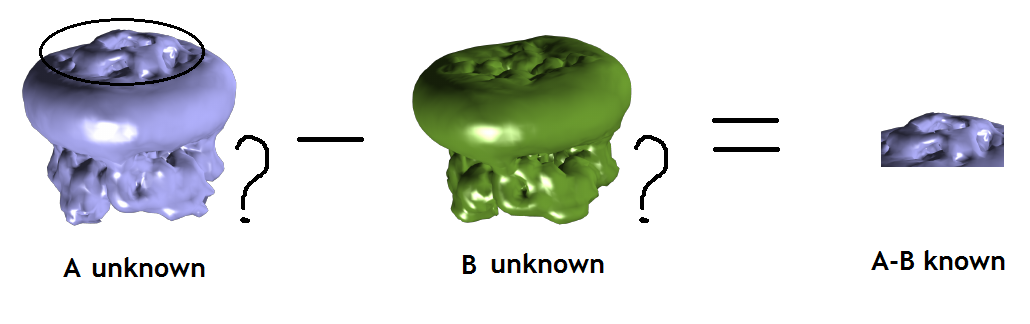
\includegraphics[width=.9\columnwidth]{figures/or_flow_q.png}
\end{figure}
\end{frame}


\begin{frame}<beamer>
\frametitle{Orthogonal Replacement (OR) \blfootnote{TB, T. Zhang, A. Singer (2015)}}
\begin{itemize}
\item $\Phi_A-\Phi_B$, cryo-EM images of $\Phi_A$ and $\Phi_B$
\end{itemize}
\begin{figure}[t]
  \centering
  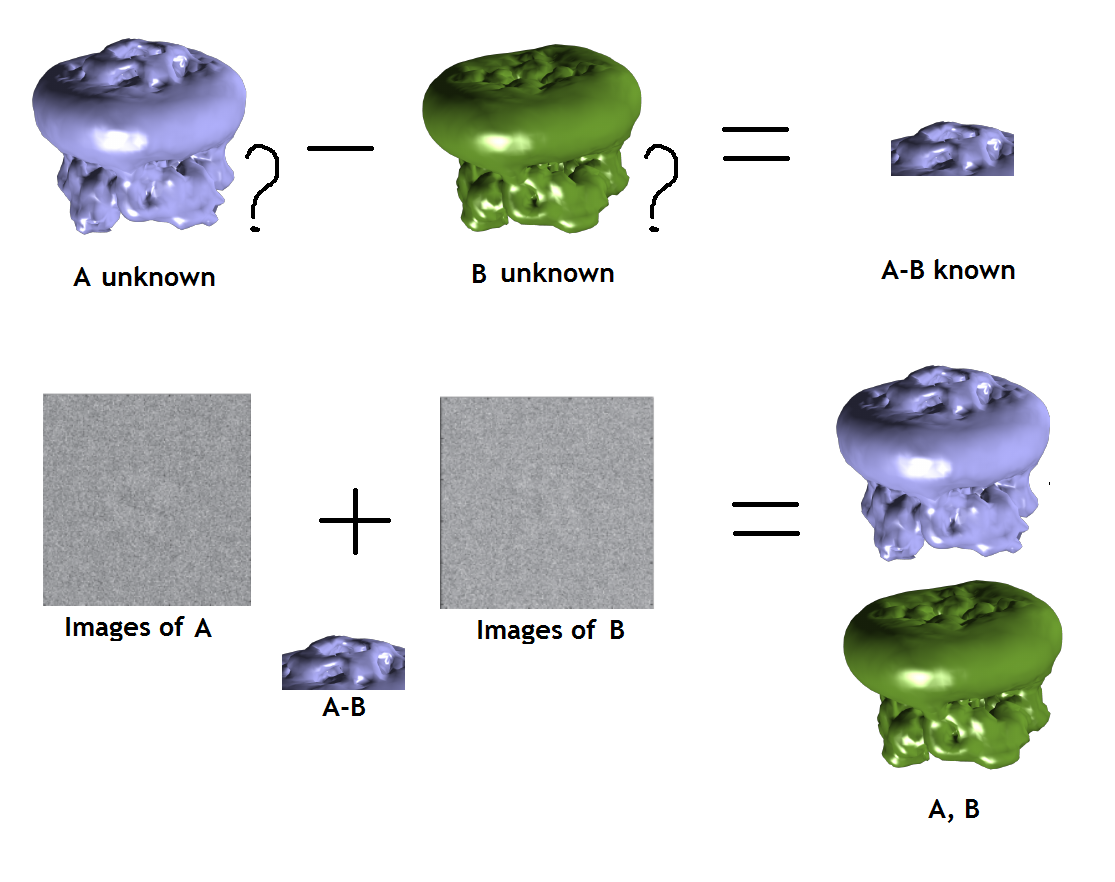
\includegraphics[width=.75\columnwidth]{figures/or_flow.png}
\end{figure}
\end{frame}


\begin{frame}<beamer>
\frametitle{Orthogonal Replacement (OR) \blfootnote{TB, T. Zhang, A. Singer (2015)}}
\begin{itemize}
\item No need for homologous structure
\item More information
\item Known structure $\Delta \Phi = \Phi_B-\Phi_A$, cryo-EM images of $\Phi_A$, $\Phi_A$
\item $\bF_{\bl}^{(A)}$ and $\bF_{\bl}^{(B)}$ computed from the autocorrelation matrix (using 2D covariance matrix from cryo-EM images)
\item Difference exactly known, unlike OE ($\bA_{\boldsymbol{l}} \approx \bB_{\boldsymbol{l}}$)
\end{itemize}
\begin{equation*}\label{lin}
\bA_{\bl}^{(B)}-\bA_{\bl}^{(A)}={\bF}_{\bl}^{(B)}\bO_{\bl}^{(B)}-\bF_{\bl}^{(B)}\bO_{\bl}^{(A)} \nonumber
\end{equation*}
\end{frame}


\begin{frame}<beamer>
\frametitle{Least Squares Problem \blfootnote{TB, T. Zhang, A. Singer (2015)}}
\begin{equation*}\label{noncon}
\min_{\bO_{\bl}^{(A)},\bO_{\bl}^{(A)} \in \text{O}(2l+1)}
\left\|\bA_{\bl}^{(B)}-\bA_{\bl}^{(A)}-{\bF}_{\bl}^{(B)}\bO_{\bl}^{(B)}+{\bF}_{\bl}^{(A)}\bO_{\bl}^{(A)} \right\|_F^2 \nonumber
\end{equation*}
\begin{itemize}
\item Non-convex
\item No closed form solution
\end{itemize}
\end{frame}

\begin{frame}<beamer>
\frametitle{Relaxation to a Semidefinite Program (SDP) \blfootnote{TB, T. Zhang, A. Singer (2015)}}
%

\begin{equation*}
\begin{aligned}
& \underset{\bQ}{\text{minimize}}
& & \mathrm{Tr}(\bW\bQ) \\
& \text{subject to}
&& \bQ \in \mathbb{R}^{3(2l+1) \times 3(2l+1)}, \\
&&&  \bQ_{ii} = \bI, \\
&&& \text{rank}(\bQ) = 2l+1, \\
&&& \bQ \succeq 0.
\end{aligned}
\end{equation*}

\begin{itemize}
\item $\bW$ can be written in terms of $\bA_{\bl}^{(B)}-\bA_{\bl}^{(A)}$,
$\bF_{\bl}^{(A)}$ and $\bF_{\bl}^{(B)}$
\item Relax rank constraint: SDP (polynomial time in $l$)
\item Round solution to rank $2l+1$
\end{itemize}

\end{frame}

%
\begin{frame}<beamer>
\frametitle{Preliminary Result: Kv1.2 Potassium Channel}
Synthetic images with SNR$=0.7, 0.35$ (\textbf{no CTF}) \blfootnote{TB, T. Zhang, A. Singer (2015)}
\begin{figure}[!htbp]
\begin{center}
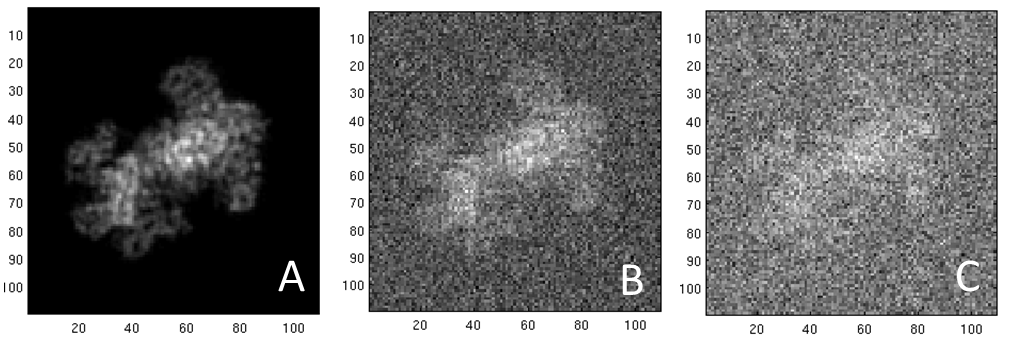
\includegraphics[width=.65 \columnwidth]{figures/proj_all.png}
\end{center}
\end{figure}
\end{frame}

\begin{frame}<beamer>
\frametitle{Preliminary Result: Kv1.2 Potassium Channel}
Clean synthetic images (\textbf{no CTF}) \blfootnote{TB, T. Zhang, A. Singer (2015)}
\begin{figure}[!htbp]
\begin{center}
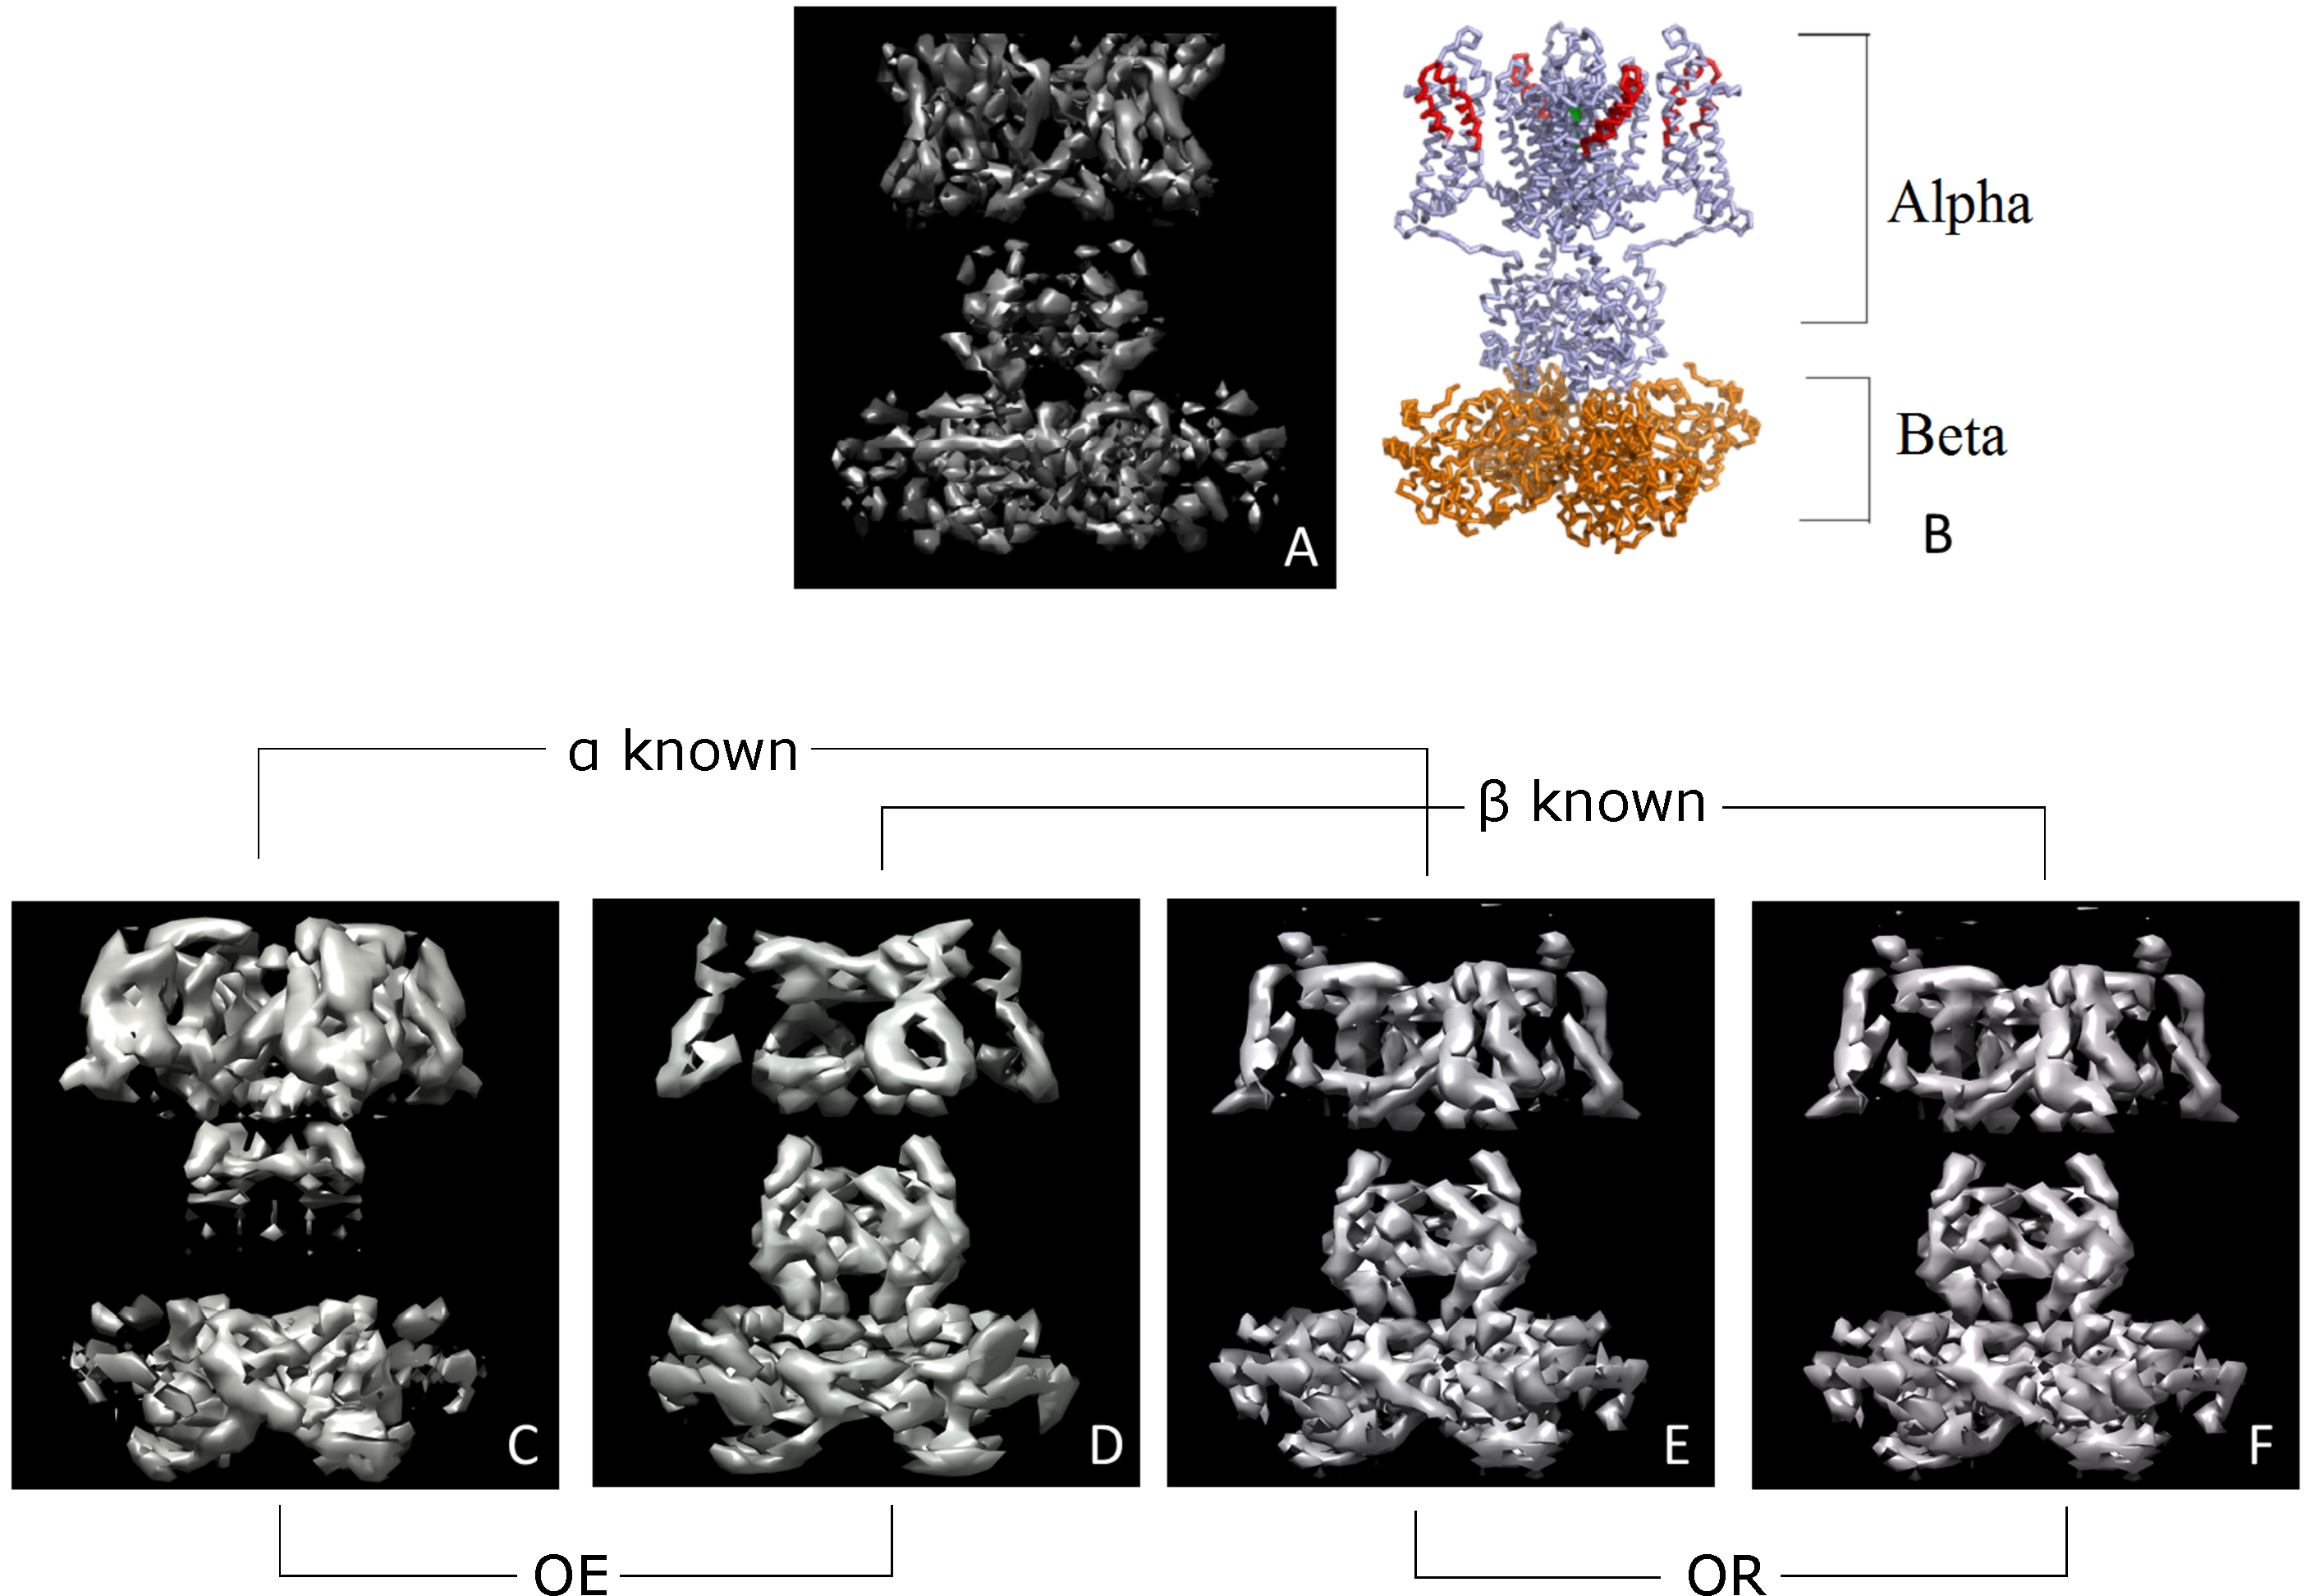
\includegraphics[width=.65 \columnwidth]{figures/reconstruction_all_clean.pdf}
\end{center}
\end{figure}
\end{frame}

\begin{frame}<beamer>
\frametitle{Preliminary Result: Kv1.2 Potassium Channel}
OR with noisy, synthetic images (\textbf{no CTF}) \blfootnote{TB, T. Zhang, A. Singer (2015)}
\begin{figure}[!htbp]
\begin{center}
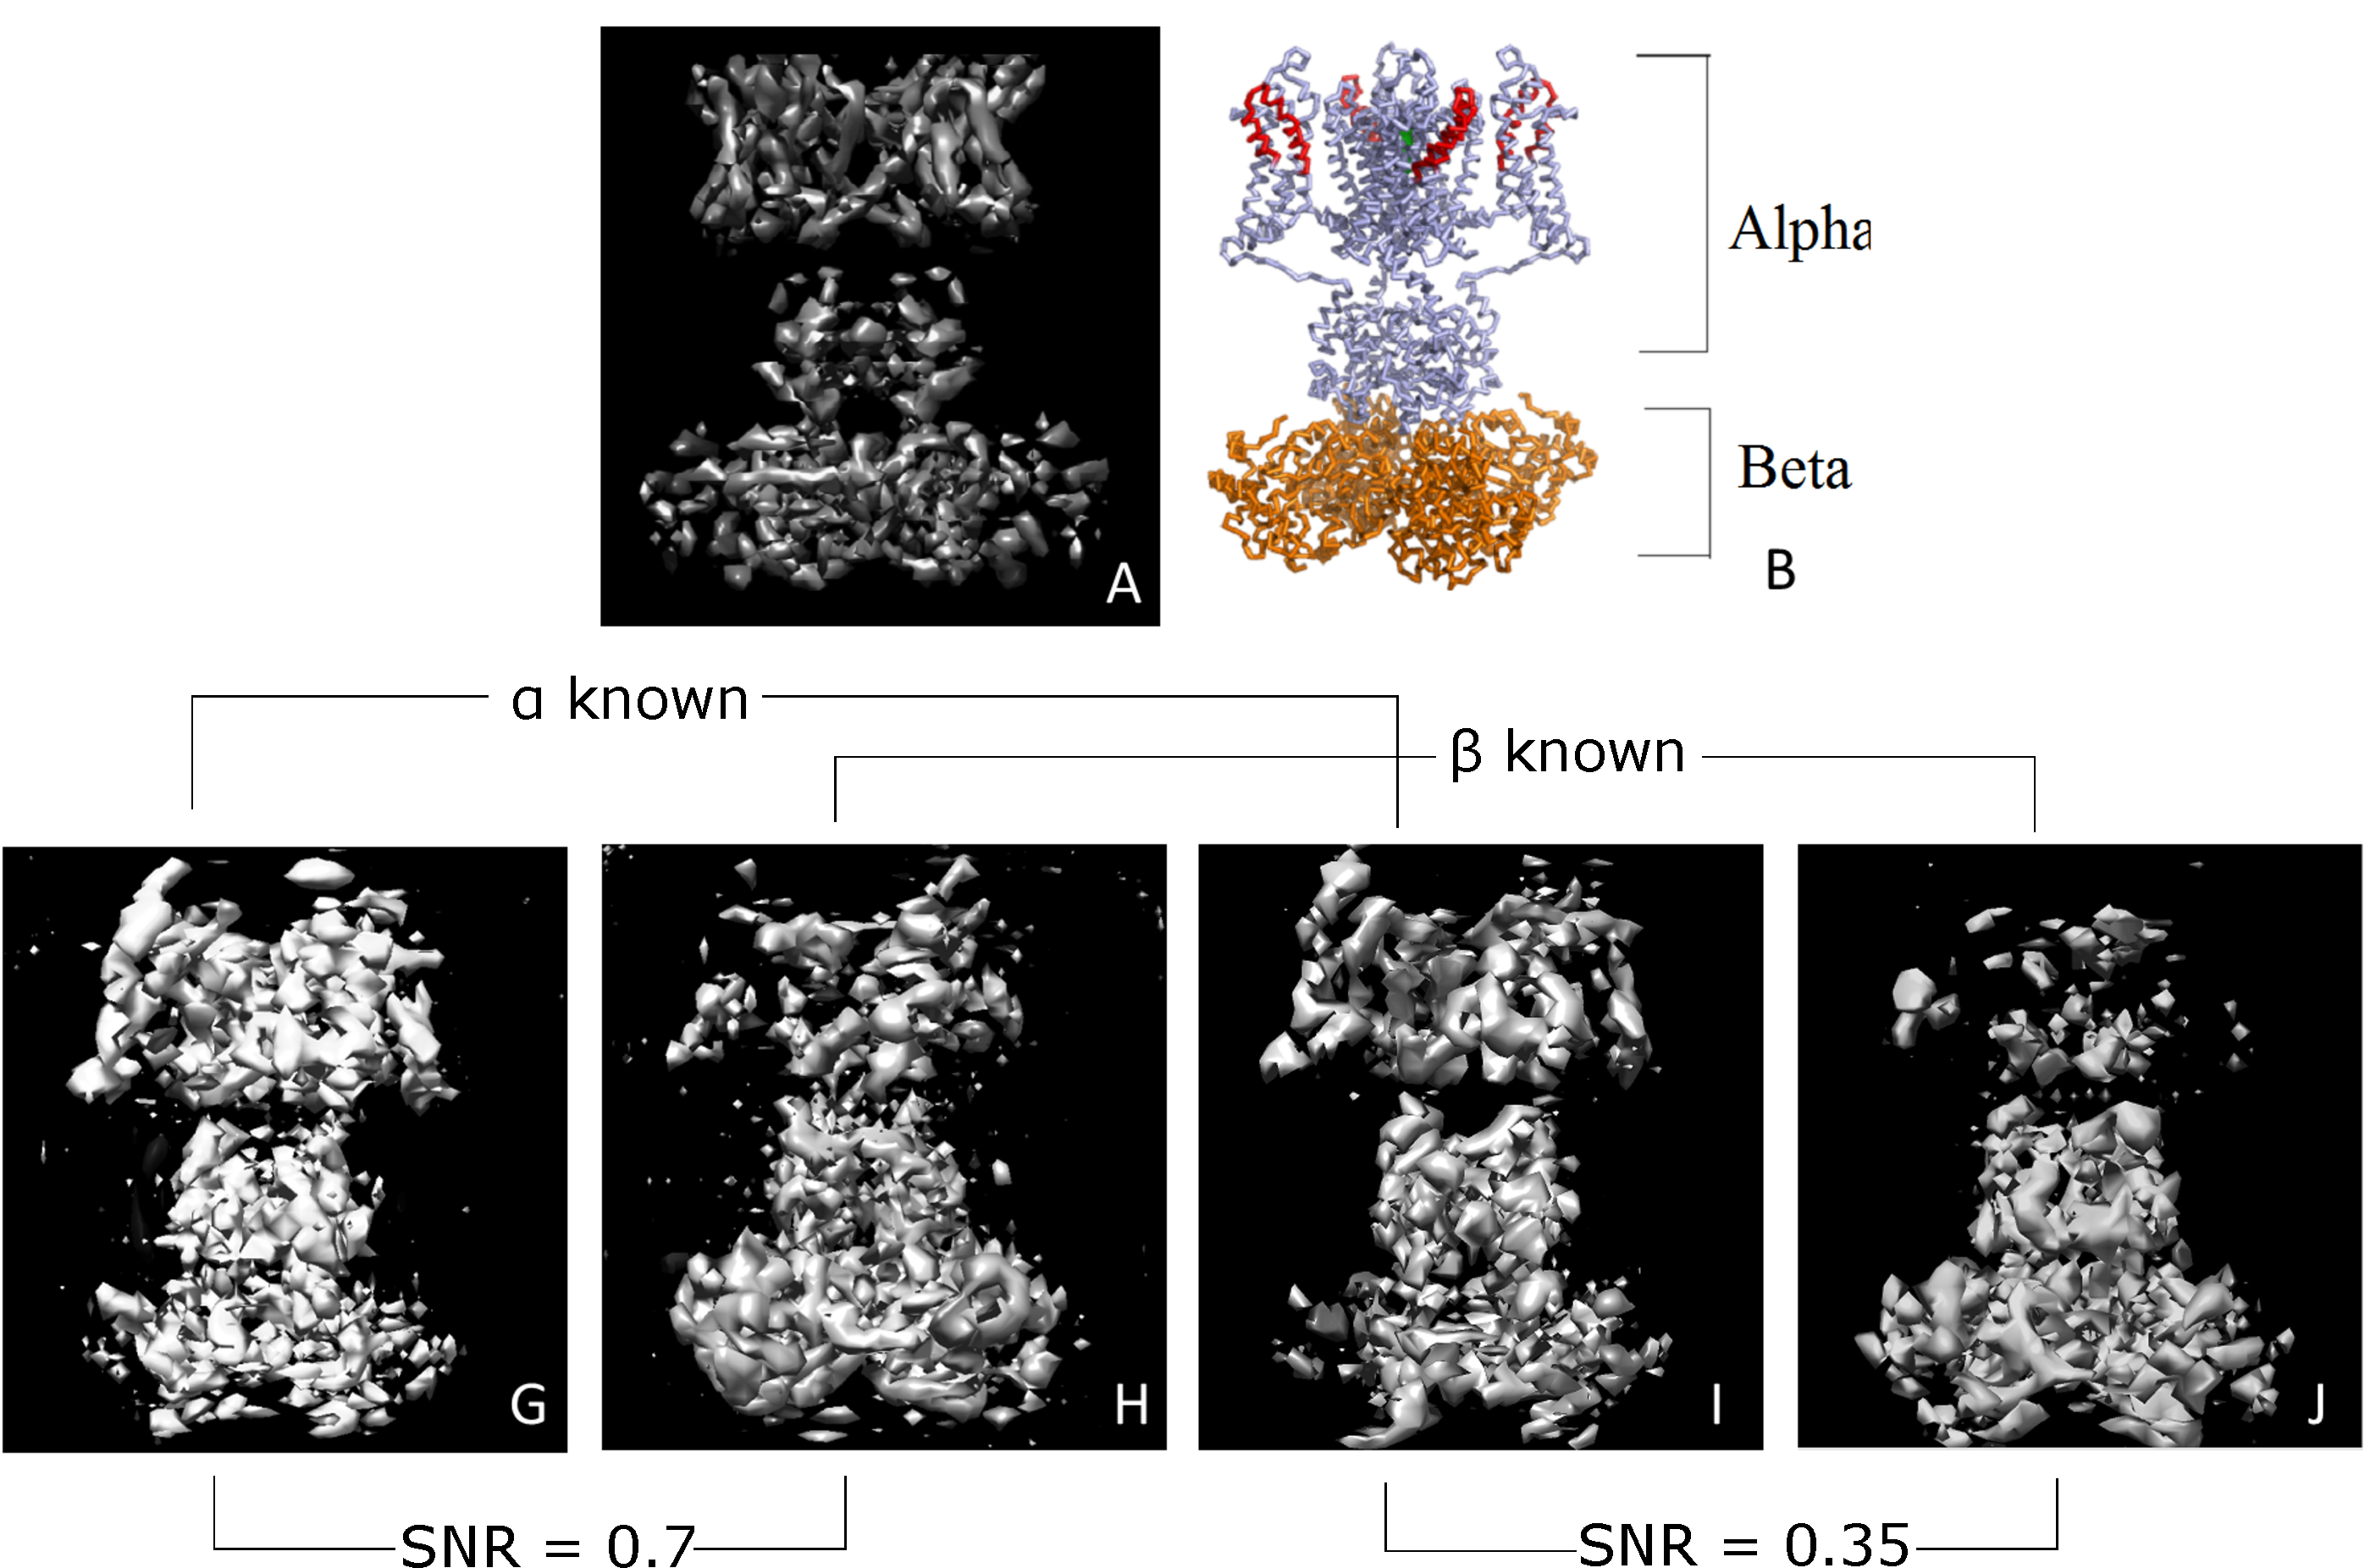
\includegraphics[width=.65 \columnwidth]{figures/reconstruction_all_noisy.pdf}
\end{center}
\end{figure}
\end{frame}

\begin{frame}<beamer>
\frametitle{Validation: Fourier Cross Resolution}
OR performs better due to addition information \blfootnote{TB, T. Zhang, A. Singer (2015)}
\begin{figure}[t]
  \centering
  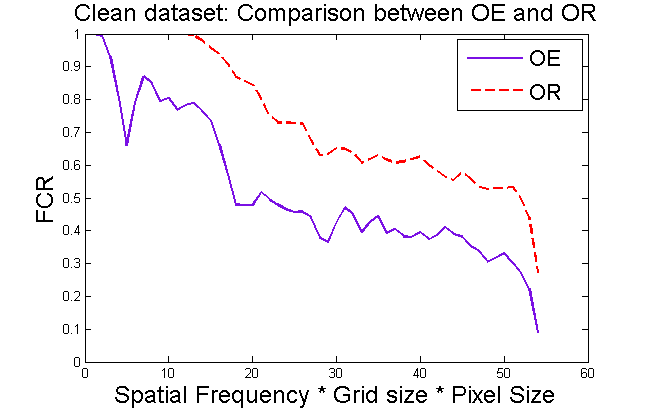
\includegraphics[width=.8\columnwidth]{figures/FSC_final.png}
  \caption{FCR curve for reconstruction from $\beta_4$ (clean images)}\label{fig:fsc}
\end{figure}
\end{frame}


\begin{frame}<beamer>
\frametitle{Revisiting OE}
 \begin{columns}
\column{0.5\linewidth}
\begin{figure}[!htbp]
\begin{center}
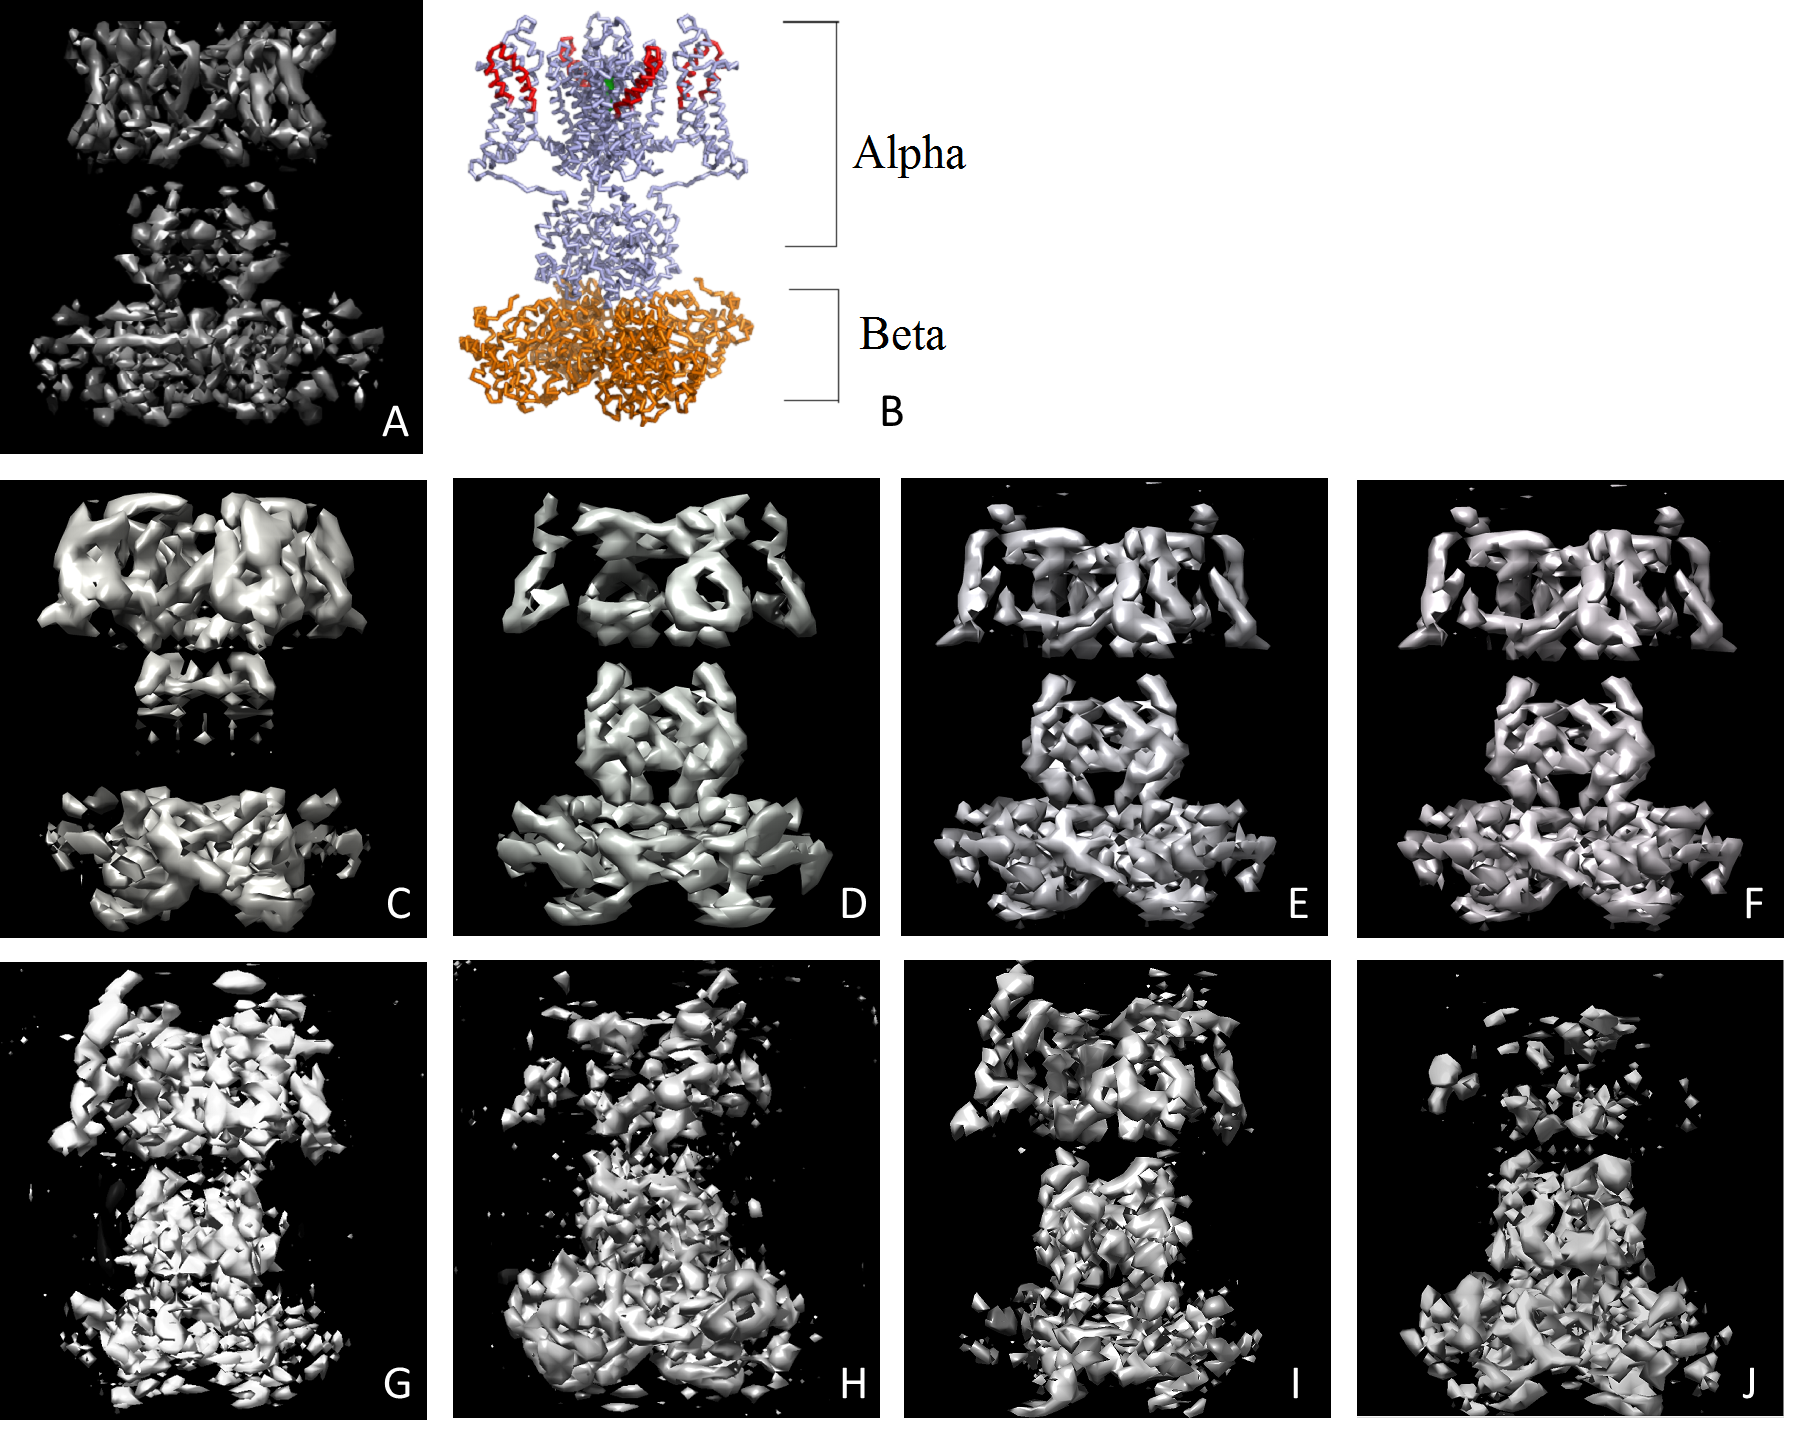
\includegraphics[width=.95 \columnwidth]{figures/reconstruction_all.png}
\end{center}
\end{figure}
\column{0.5\linewidth} 
\begin{itemize}
\item Preliminary result: no CTF
\item Expect improvement using estimated covariance $\Sigma$
\item Test on real data with CTF and low SNR
\end{itemize}
\end{columns}
\end{frame}

\begin{frame}<beamer>
\frametitle{Revisiting OE: Unbiased Estimator}
 \begin{columns}
\column{0.5\linewidth}
\centering
\begin{tabular}{cc}
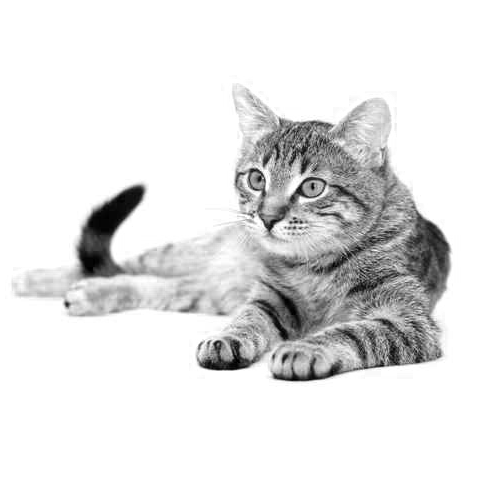
\includegraphics[width=0.35\linewidth]{figures/cat.png}
&\includegraphics[width=0.35\linewidth]{figures/cat_tail.png}\\
\includegraphics[width=0.35\linewidth]{figures/cat_t1.png}
&\includegraphics[width=0.35\linewidth]{figures/cat_t2.png}\\
\end{tabular}
\column{0.5\linewidth} 
\begin{itemize}
\item Twicing $2\hat{\bA}_{\text{LS}}-\bB$: unbiased estimator for scalar case $\bA\in\mathbb{C}^{1\times 1}$
\item Recovers unknown subunit better 
\item How to estimate
$\bA \in\mathbb{R}^{N\times D}$ (or $\mathbb{C}^{N\times D}$) from $\bC$ and
$\bB$, where $\bC=\bA \bA^*$ and $\bA=\bB+\bE$ for a matrix $\bE$ of small
magnitude?
\end{itemize}
\end{columns}
\end{frame}

\begin{frame}<beamer>
\frametitle{Unbiased Estimator: Anisotropic Twicing (AT)}
\begin{itemize}
\item Spectral decomposition $\bC=\bU\diag(\lambda_1,\lambda_2,\cdots,\lambda_D)\bU^*$
\item Asymptotically unbiased estimator \blfootnote{TB, T. Zhang, A. Singer (2017+)} of $\bA$ when $N=D$ is given by
\end{itemize}

\begin{equation*}
\hat{\bA}_{\text{AT}}=\bB+\bU\bW\bU^*(\hat{\bA}_{\text{LS}}-\bB) \nonumber
\end{equation*}
where 
$\bT$ is a diagonal matrix with
$\bT_{ii}=\begin{cases}\frac{1}{D}\Big[-\frac{1}{2}+\sum_{1\leq j\leq 
D}\frac{\lambda_i^2}{\lambda_i^2+\lambda_j^2}\Big]\,\,\,\text{when 
$\bA,\bC\in\mathbb{R}^{D\times D}$},\\\frac{1}{D}\sum_{1\leq j\leq 
D}\frac{\lambda_i^2}{\lambda_i^2+\lambda_j^2}
\,\,\,\text{when $\bA,\bC\in\mathbb{C}^{D\times D}$},
\end{cases}$\\
and $\bW=(\bI-\bT)^{-1}$
%\begin{itemize}
%\item Family of estimators
%\end{itemize}

\end{frame}


\begin{frame}<beamer>
\frametitle{Unbiased Estimator: Anisotropic Twicing (AT) }
\begin{equation*}
\label{eqn:biasvar}
\text{MSE}=\mathbb{E}[||\theta-\hat{\theta}||^2] = ||\text{Bias}||^2 + \text{Var} \nonumber
\end{equation*}
\begin{figure}[!htbp]
\begin{center}
\includegraphics[scale=0.35]{figures/anis_bias_family_few.png}
\end{center}
\end{figure}\blfootnote{TB, T. Zhang, A. Singer (2017+)}
\end{frame}

\begin{frame}<beamer>
\frametitle{Synthetic Dataset: Toy Molecule }
$10000$, clean images\\
Relative error in unknown subunit: AT $19\%$, Twicing $31\%$, LS $59\%$ 
\begin{figure}[!htbp]
\begin{center}
\includegraphics[scale=0.16]{figures/mickey.pdf}
\end{center}
\end{figure}\blfootnote{TB, T. Zhang, A. Singer (2017+)}

\end{frame}

\begin{frame}<beamer>
\frametitle{Synthetic Dataset: TRPV1 }
SNR$=1/40$, $26000$ images, $10$ defocus groups.\\ 
Relative error in unknown subunit: AT $30\%$, Twicing $56\%$, LS $43\%$ 
\begin{figure}[!htbp]
\begin{tabular}{cc}
\includegraphics[width=0.4\linewidth]{figures/sim8117_compare.pdf}\label{fig:simtrpv_emdb} \\
\includegraphics[width=0.9\linewidth]{figures/sim8117.pdf}\label{fig:simtrpv_res}\\
\end{tabular}
\end{figure}\blfootnote{TB, T. Zhang, A. Singer (2017+)}

\end{frame}


\begin{frame}<beamer>
\frametitle{Experimental Dataset: TRPV1 with DkTx and RTx }
EMPIAR 10059: $73000$ motion corrected images
\begin{figure}[]
\label{fig:realtrpv}
\centering
\begin{tabular}{cc}
\includegraphics[width=0.5\linewidth]{figures/realdat_unif1.pdf} \\
Non-uniform viewing angles \\ 
\includegraphics[width=0.5\linewidth]{figures/realdat_unif0.pdf}\\
Selecting $\sim 30000$ uniform viewing angles
\end{tabular}
\end{figure}\blfootnote{TB, T. Zhang, A. Singer (2017+)}
\alert{Robust to viewing angle distribution}
\end{frame}


\begin{frame}<beamer>
\frametitle{Validation: FCR }
Dataset: EMPIAR 10059
\begin{figure}[]
\caption{}
\centering
\begin{tabular}{cc}
\includegraphics[width=0.45\linewidth]{figures/realdat_109_fsc.png}
&\includegraphics[width=0.45\linewidth]{figures/realdat_109ball_fsc.png}\\
Full volume & Unknown subunit\\
\end{tabular}\blfootnote{TB, T. Zhang, A. Singer (2017+)}
\end{figure}
\end{frame}


\begin{frame}<beamer>
\frametitle{Advantage of Autocorrelation Analysis}
\begin{itemize}
\item Covariance matrix computation: $O(n)$
\item Single refinement iteration: comparison of pairs of images
\item Good starting model can significantly reduce refinement iterations
\end{itemize}
\end{frame}

\begin{frame}<beamer>
\frametitle{Summary}
\begin{itemize}
\item \textbf{Covariance estimation}: denoising, CTF correction, outlier detection
\item \textbf{Homology modeling}: 3D model directly from raw data
\end{itemize}
\end{frame}


\begin{frame}<beamer>
\frametitle{Other applications}
\begin{itemize}
\item \textbf{Covariance estimation}: other kinds of data with or without blurring kernels
\item \textbf{Homology modeling}: 3D model directly from raw data
\item Model validation
\item Extension to SPR with X-ray free electron lasers (XFEL)
\end{itemize}
\end{frame}

\begin{frame}<beamer>
\frametitle{Acknowledgement}
\begin{columns}
\column{0.5\linewidth} 
Amit Singer (Princeton)\\
David Huse (Princeton)\\
Fred Sigworth (Yale)\\
Joakim Anden (Princeton)\\
Joshua Shaevitz (Princeton)\\
Paul Steinhardt (Princeton)\\
Teng Zhang (UCF)\\
Xiuyuan Cheng (Yale)\\
Yoel Shkolnisky (Tel-Aviv) \\
Zhizhen Zhao (UIUC)\\

\column{0.5\linewidth} 
Adam Frost (UCSF)\\
Daniel Asarnow (UCSF)\\
David Julius (UCSF)\\
Eugene Palovcak (UCSF)\\
Garib Murshudov (MRC Cambridge)\\
Xiaochen Bai (UTS)\\
Yuan Gao (UCSF)\\

\end{columns}
\end{frame}

\section{Appendix}

\begin{frame}<beamer>
\frametitle{Simulations with colored noise: 80S ribosome (EMDB-6454)}

\begin{figure}[]
\centering
\subfloat[SNR=$1$]{\begin{overpic}[width=0.4\linewidth]{figures/compare_ims_col_snr1by1_6454.eps}
\put(6,52){\tiny Clean}
\put(32,52){\tiny Noisy}
\put(55,52){\tiny TWF}
\put(80,52){\tiny CWF}
\put(-32,35){\tiny Defocus=$1\mu m$}
\put(-32,10){\tiny Defocus=$4\mu m$}
\end{overpic}%
}
\vspace{-1mm}
\subfloat[SNR=$1/10$]{\begin{overpic}[width=0.4\linewidth]{figures/compare_ims_col_snr1by10_6454.eps}%
\end{overpic}%
\label{}}
\vspace{-1mm}
\subfloat[SNR=$1/20$]{\begin{overpic}[width=0.4\linewidth]{figures/compare_ims_col_snr1by20_6454.eps}%
\end{overpic}%
\label{}}

\label{fig:ims_6454_colored}
\end{figure}

\end{frame}


\begin{frame}<beamer>
\frametitle{Relative error of estimated clean images}

\begin{figure}[]
\centering
\subfloat[]{\begin{overpic}[width=0.5\linewidth]{figures/mse_snr_6454.eps}%
\end{overpic}%
\label{fig:mse_snr}}
\subfloat[]{\begin{overpic}[width=0.5\linewidth]{figures/mse_nims_6454.eps}
\end{overpic}
\label{fig:mse_nims}}
\caption{(a) {Fixed number of images}
(b) {Fixed SNR}
}
\end{figure}
\end{frame}
\end{document}